\documentclass{beamer}
\mode<presentation>
\usetheme{Berlin}
\usepackage{tabularx}

\title{Introduction to Soldering}
\author{Andrew D. Zonenberg}
%\institute{Antikernel Labs}
\date{\today}

\begin{document}

\frame{\titlepage}

\begin{frame}
\frametitle{About Me}

\begin{itemize}
\item 2013-2015: Process Engineer, LIB3
\item 2015: Ph.D Computer Science (RPI)
\item 2015 - present: Sr. Security Consultant, IOActive
%\item 2016 - present: Research Scientist, Antikernel Labs
\item Designing and soldering PCBs since 2009
\end{itemize}
\end{frame}

\begin{frame}
\frametitle{What is Soldering?}
\begin{itemize}
\item Joining parts with a \emph{low melting point} filler metal
\item Reversible - filler can be removed to separate parts
\item Provides both \emph{electrical} and \emph{mechanical} connection
\end{itemize}
\begin{center}
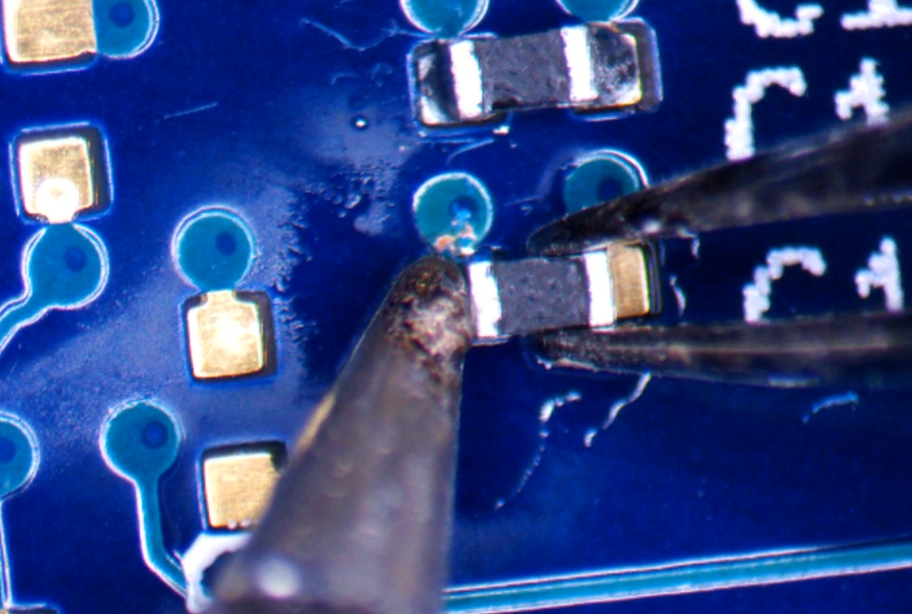
\includegraphics[height=3cm,keepaspectratio]{intro-shot.jpg}
\end{center}
\end{frame}

\begin{frame}
\frametitle{Safety Concerns}
\begin{itemize}
\item Toxic heavy metals (Pb, Cd, Sb)
\item High temperatures
\item Flux smoke
\end{itemize}
\begin{center}
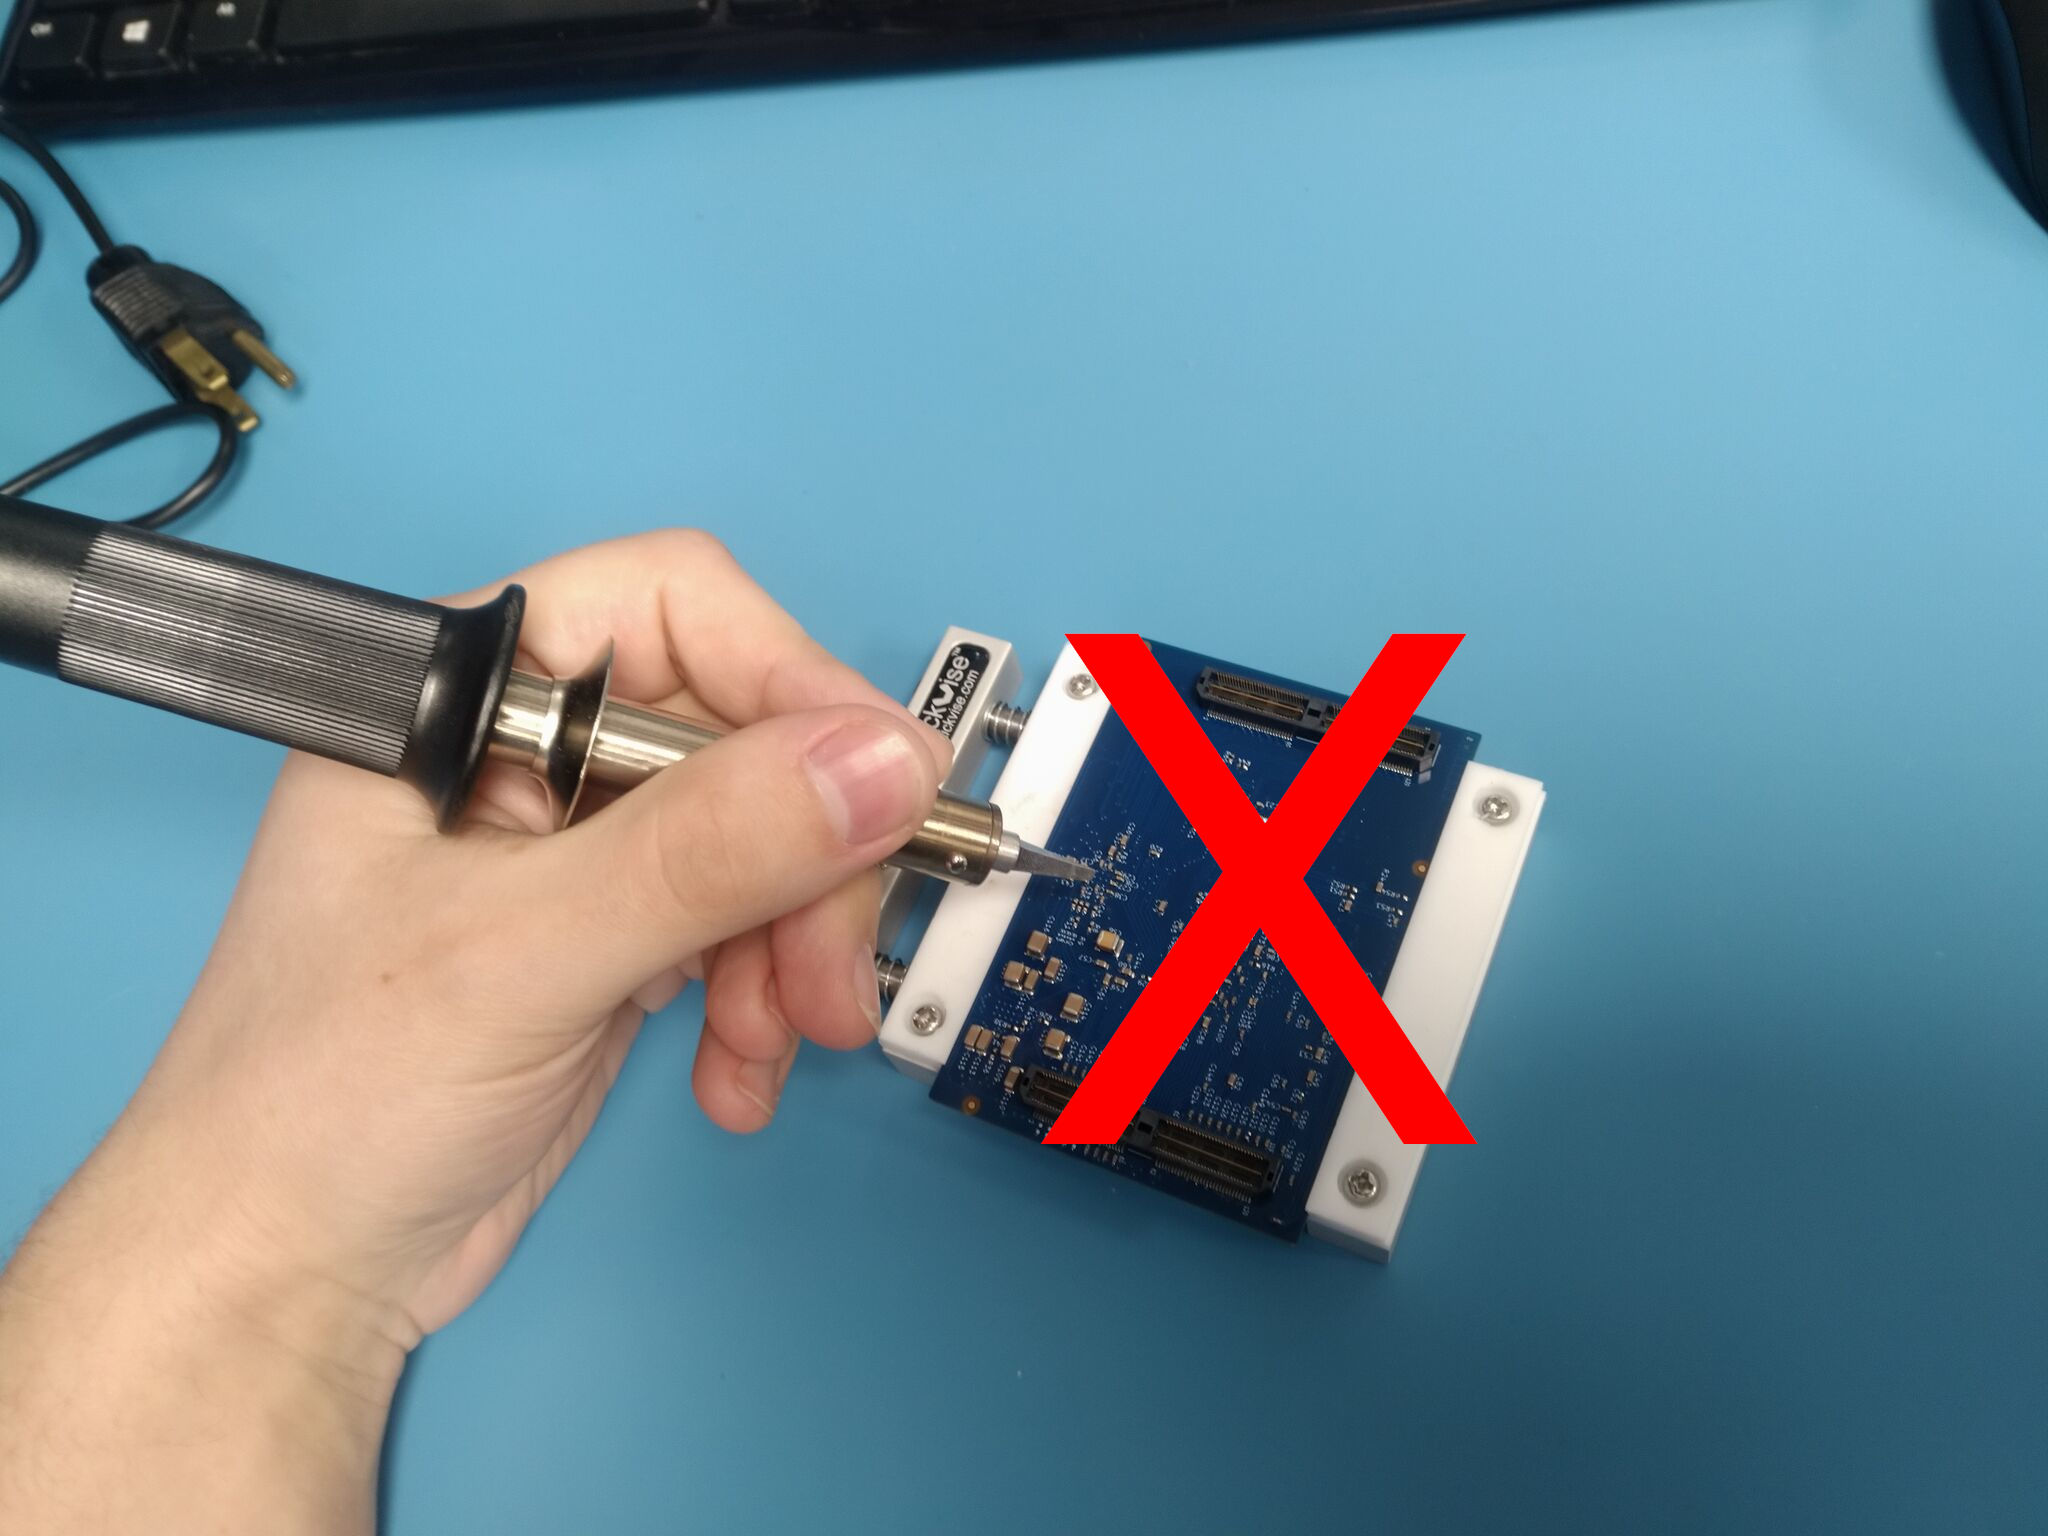
\includegraphics[width=4cm,keepaspectratio]{safety.jpg}
\end{center}
\end{frame}

\begin{frame}
\frametitle{Tin Whiskers}
\begin{itemize}
\item Metals can form ``whiskers" over time, causing shorts
\item Exact mechanism of formation not well understood
\item Addition of lead to tin reduces whisker formation
\item Mostly a concern in aerospace / life safety systems
\end{itemize}
\begin{center}
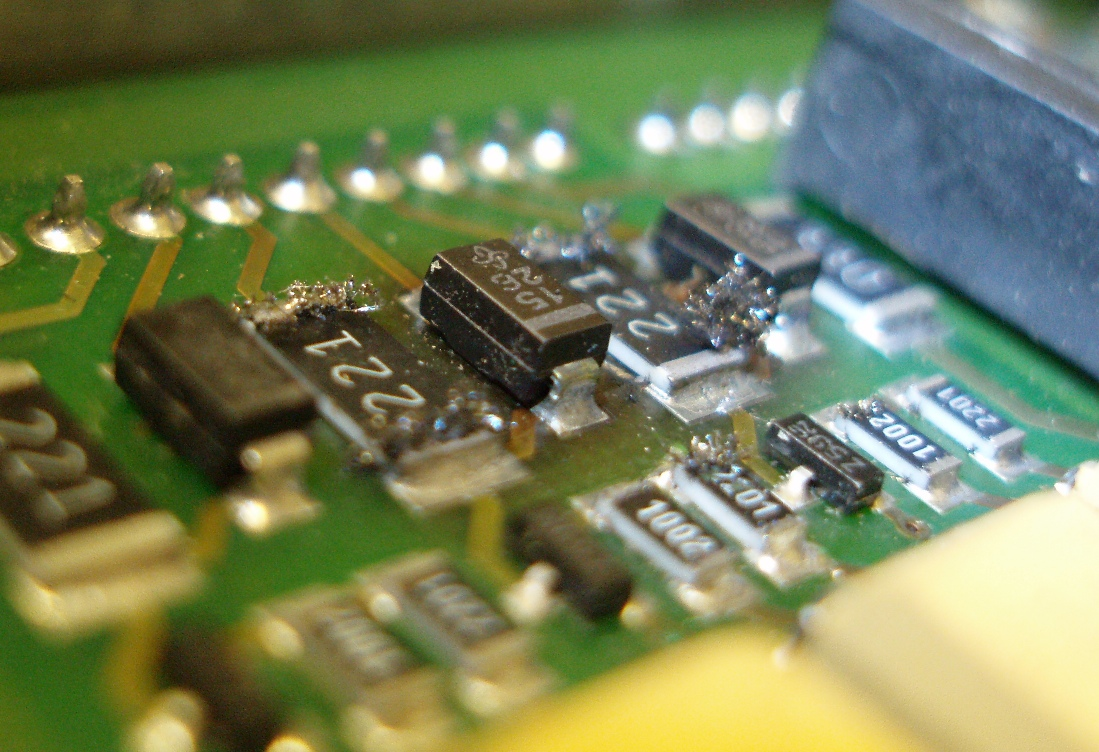
\includegraphics[width=4cm,keepaspectratio]{whiskers.jpg}
\end{center}
\end{frame}

\begin{frame}
\frametitle{Sn-Pb Solder Alloys}
\begin{itemize}
\item Largely immune to tin whiskers
\item Midrange melting point (183C for 63/37 eutectic)
\item Industry standard until early 2000s
\item Banned in Europe since 2003 due to toxicity
\item Still used in some medical/aerospace applications
\end{itemize}
\begin{alertblock}{Safety note}
Lead is a cumulative neurotoxin! Wash hands after handling lead-based solder.
\end{alertblock}
\end{frame}

\begin{frame}
\frametitle{SAC Solder Alloys (Sn-Ag-Cu)}
\begin{itemize}
\item 3\% Ag / 0.5\% Cu is most common
\item Not eutectic, but close
\item Higher melting point (SAC305 is 217-220C)
\item Nontoxic
\item Susceptible to tin whiskers
\end{itemize}
\end{frame}

\begin{frame}
\frametitle{Low Melting Point Alloys}
\begin{itemize}
\item Used on heat-sensitive components (LED lighting etc)
\item Brittle, lose strength when heated
\end{itemize}

\begin{tabularx}{\textwidth}{| X | X |}
\hline
\textbf{Alloy} & \textbf{Melting point}	\\ \hline
52\% In / 48\% Sn & 118C				\\ \hline
57\% Bi / 42\% Sn / 1\% Ag & 138C		\\ \hline
100\% In & 157C							\\ \hline
\end{tabularx}
\end{frame}

\begin{frame}
\frametitle{PCB Surface Finishes}
\begin{itemize}
\item Bare copper corrodes rapidly
\item Protective layer is applied to pads at the factory
\item SMOBC (Solder Mask Over Bare Copper)
\end{itemize}
\begin{center}
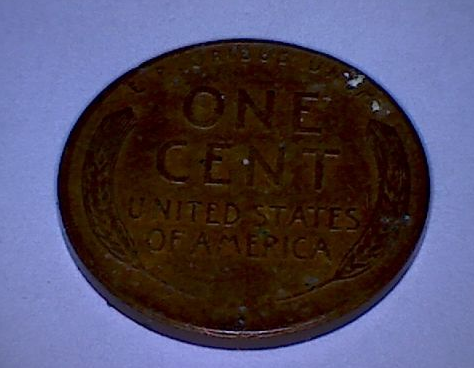
\includegraphics[width=4cm,keepaspectratio]{oxidized-copper.jpg}
\end{center}
\end{frame}

\begin{frame}
\frametitle{Unplated Copper}
\begin{itemize}
\item Extremely short shelf life
\item Only used in low cost, quick turn prototypes
\item Common on home-etched boards
\item Extremely flat surface
\end{itemize}
\begin{center}
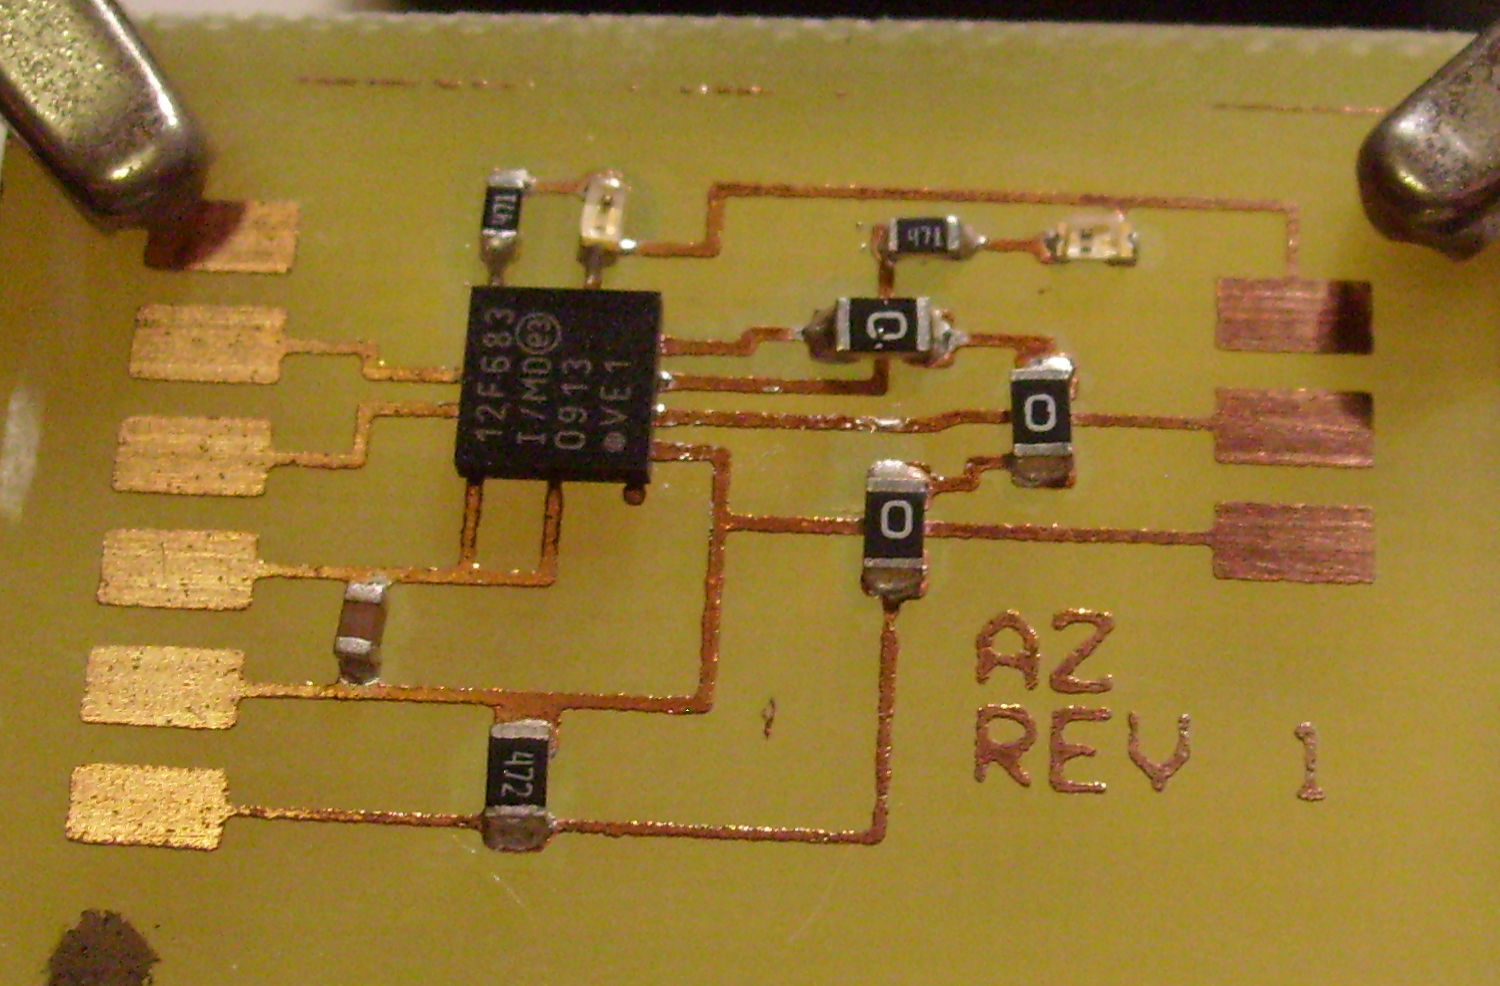
\includegraphics[width=4cm,keepaspectratio]{no-plating.jpg}
\end{center}
\end{frame}

\begin{frame}
\frametitle{HASL - Hot Air Solder Leveling}
\begin{itemize}
\item Thick (1800 - 5100 nm) layer of solder
\item Board finish \emph{is} solder - excellent solderability
\item Cheap, but poor surface flatness
\end{itemize}
\begin{center}
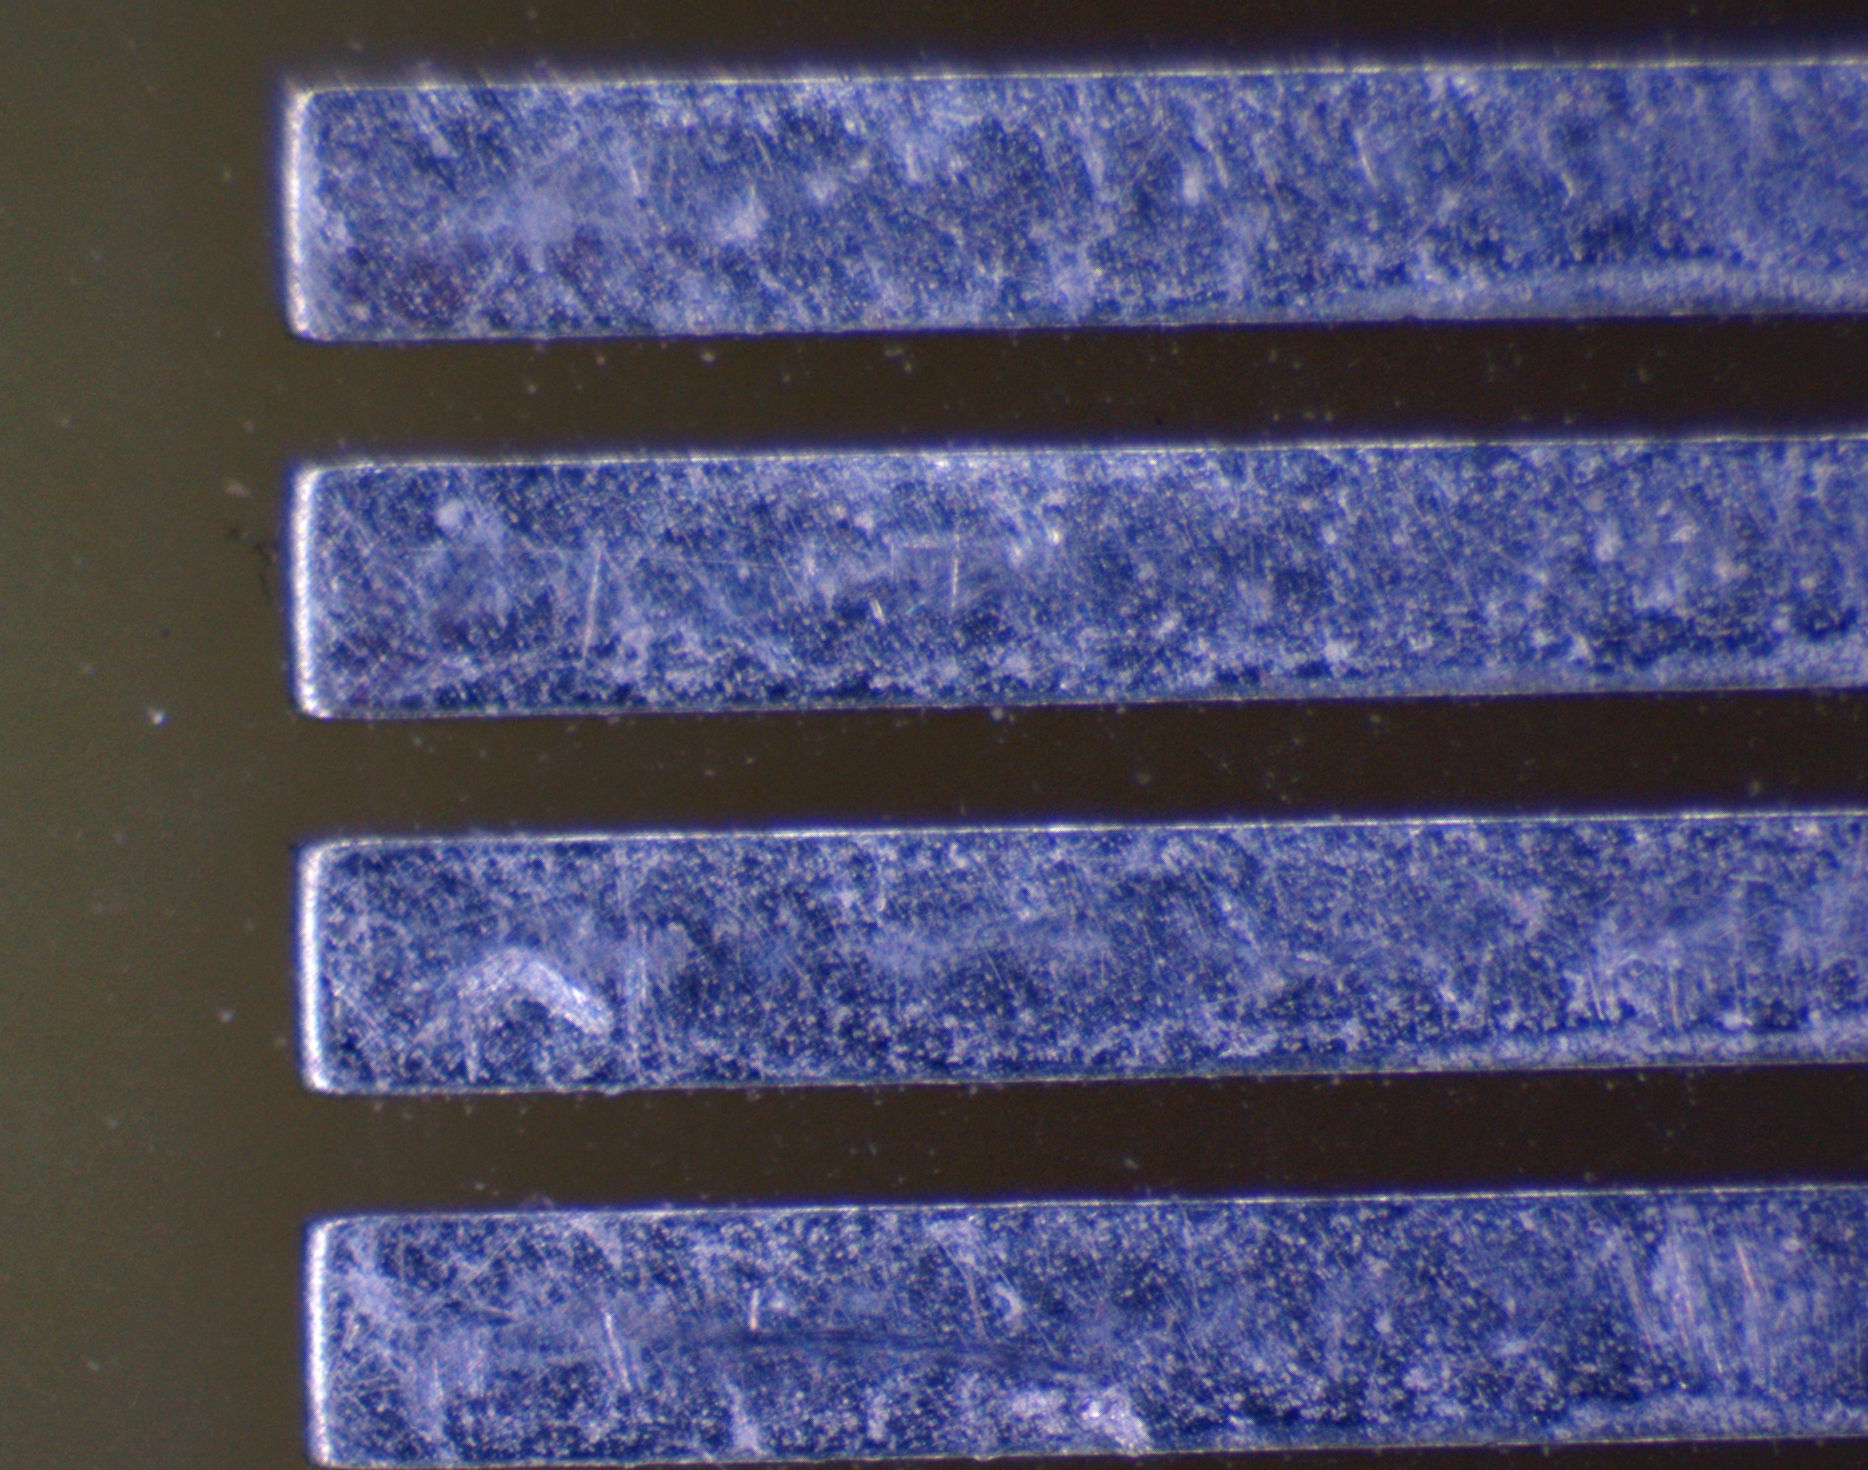
\includegraphics[height=4cm,keepaspectratio]{hasl.jpg}
\end{center}
\end{frame}

\begin{frame}
\frametitle{OSP - Organic Solderability Preservative}
\begin{itemize}
\item Very thin (200 - 500 nm) organic oxidation barrier
\item Degrades rapidly if not soldered
\item Inexpensive and extremely flat
\end{itemize}
\begin{center}
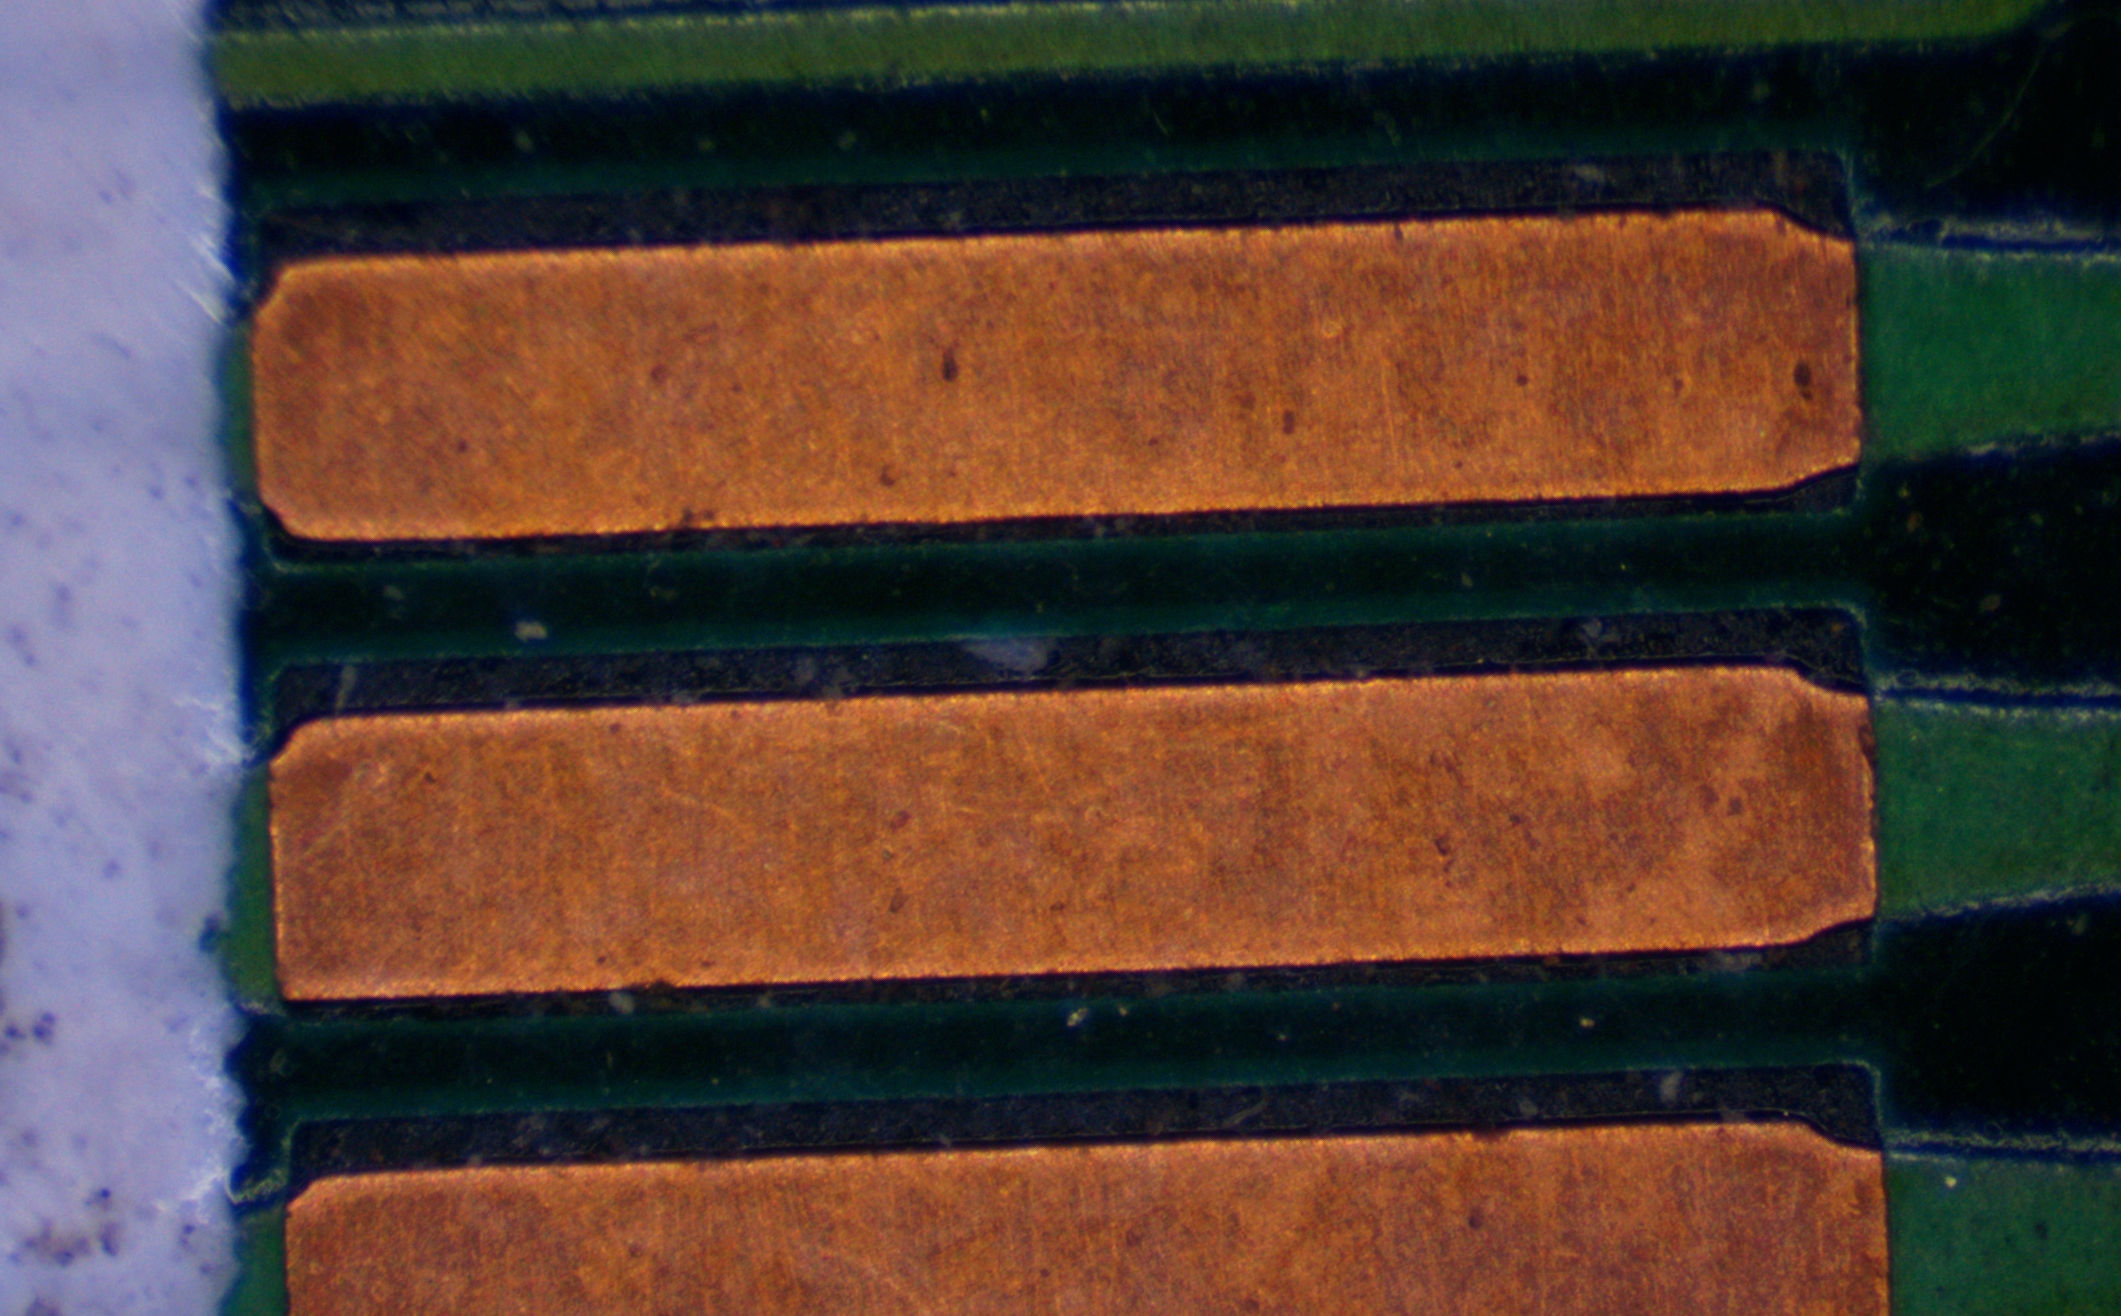
\includegraphics[height=4cm,keepaspectratio]{osp.jpg}
\end{center}
\end{frame}

\begin{frame}
\frametitle{Immersion Tin / Silver}
\begin{itemize}
\item Thicker than OSP (500 - 1200 nm)
\item Moderate shelf life
\item More expensive, but flat
\end{itemize}
\begin{center}
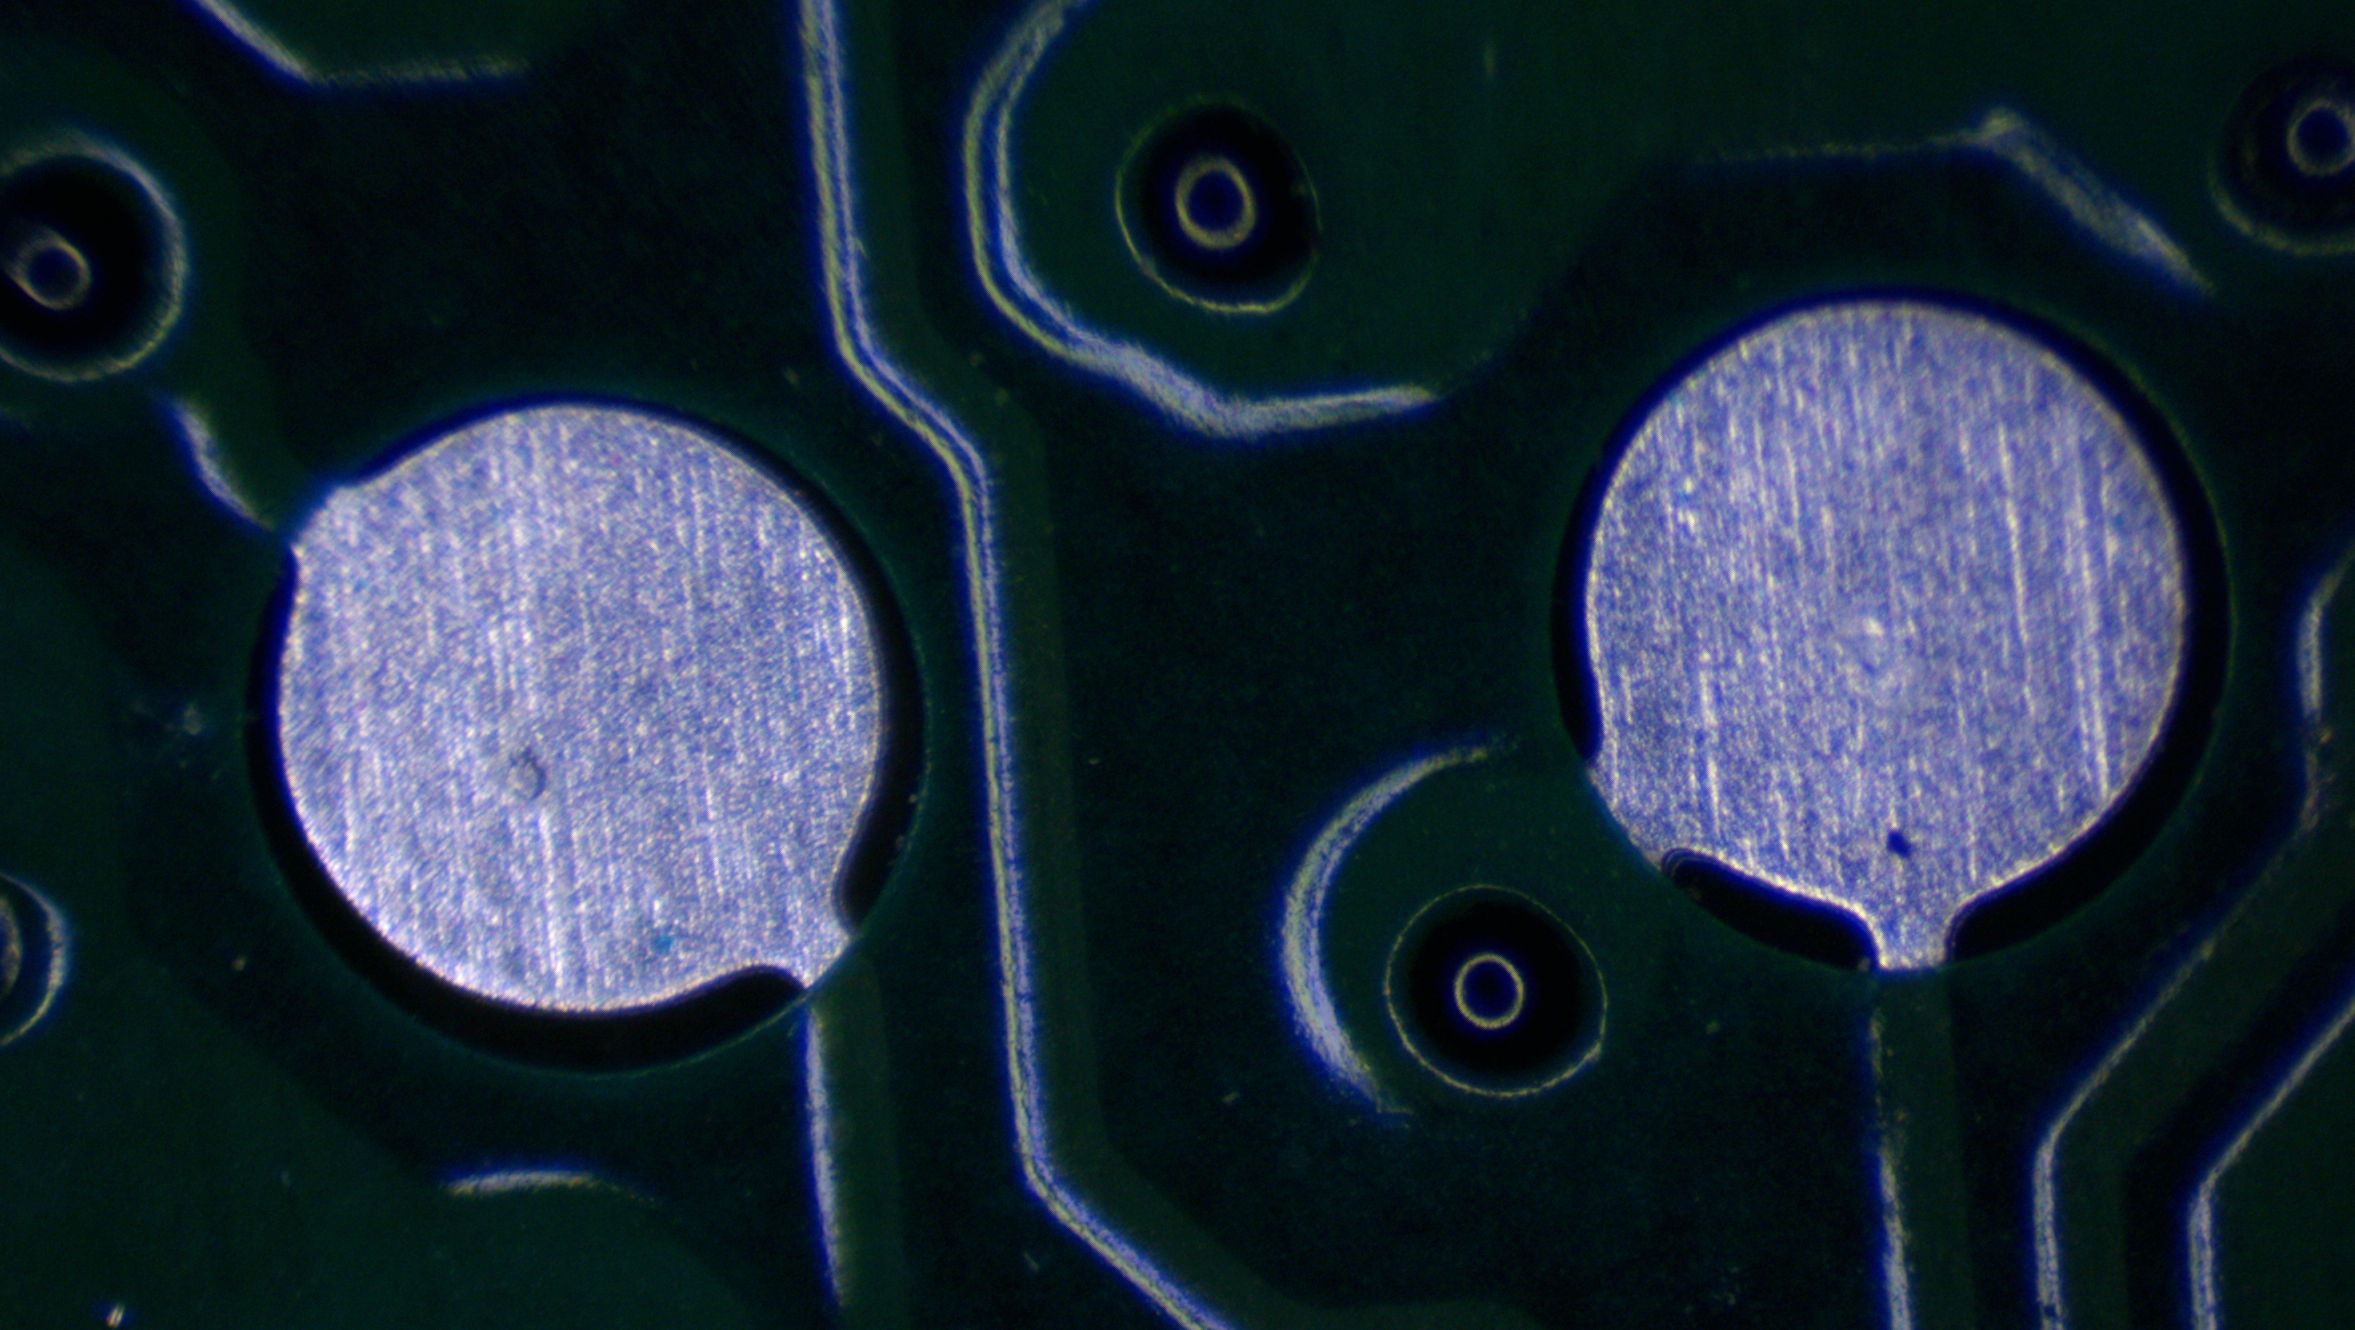
\includegraphics[height=4cm,keepaspectratio]{immersion-silver.jpg}
\end{center}
\end{frame}

\begin{frame}
\frametitle{ENIG}
\begin{itemize}
\item 2-layer system: 75-125 nm Au over 3000 - 6000 nm Ni
\item Ni acts as diffusion barrier
\item More expensive
\item Long shelf life
\end{itemize}
\begin{center}
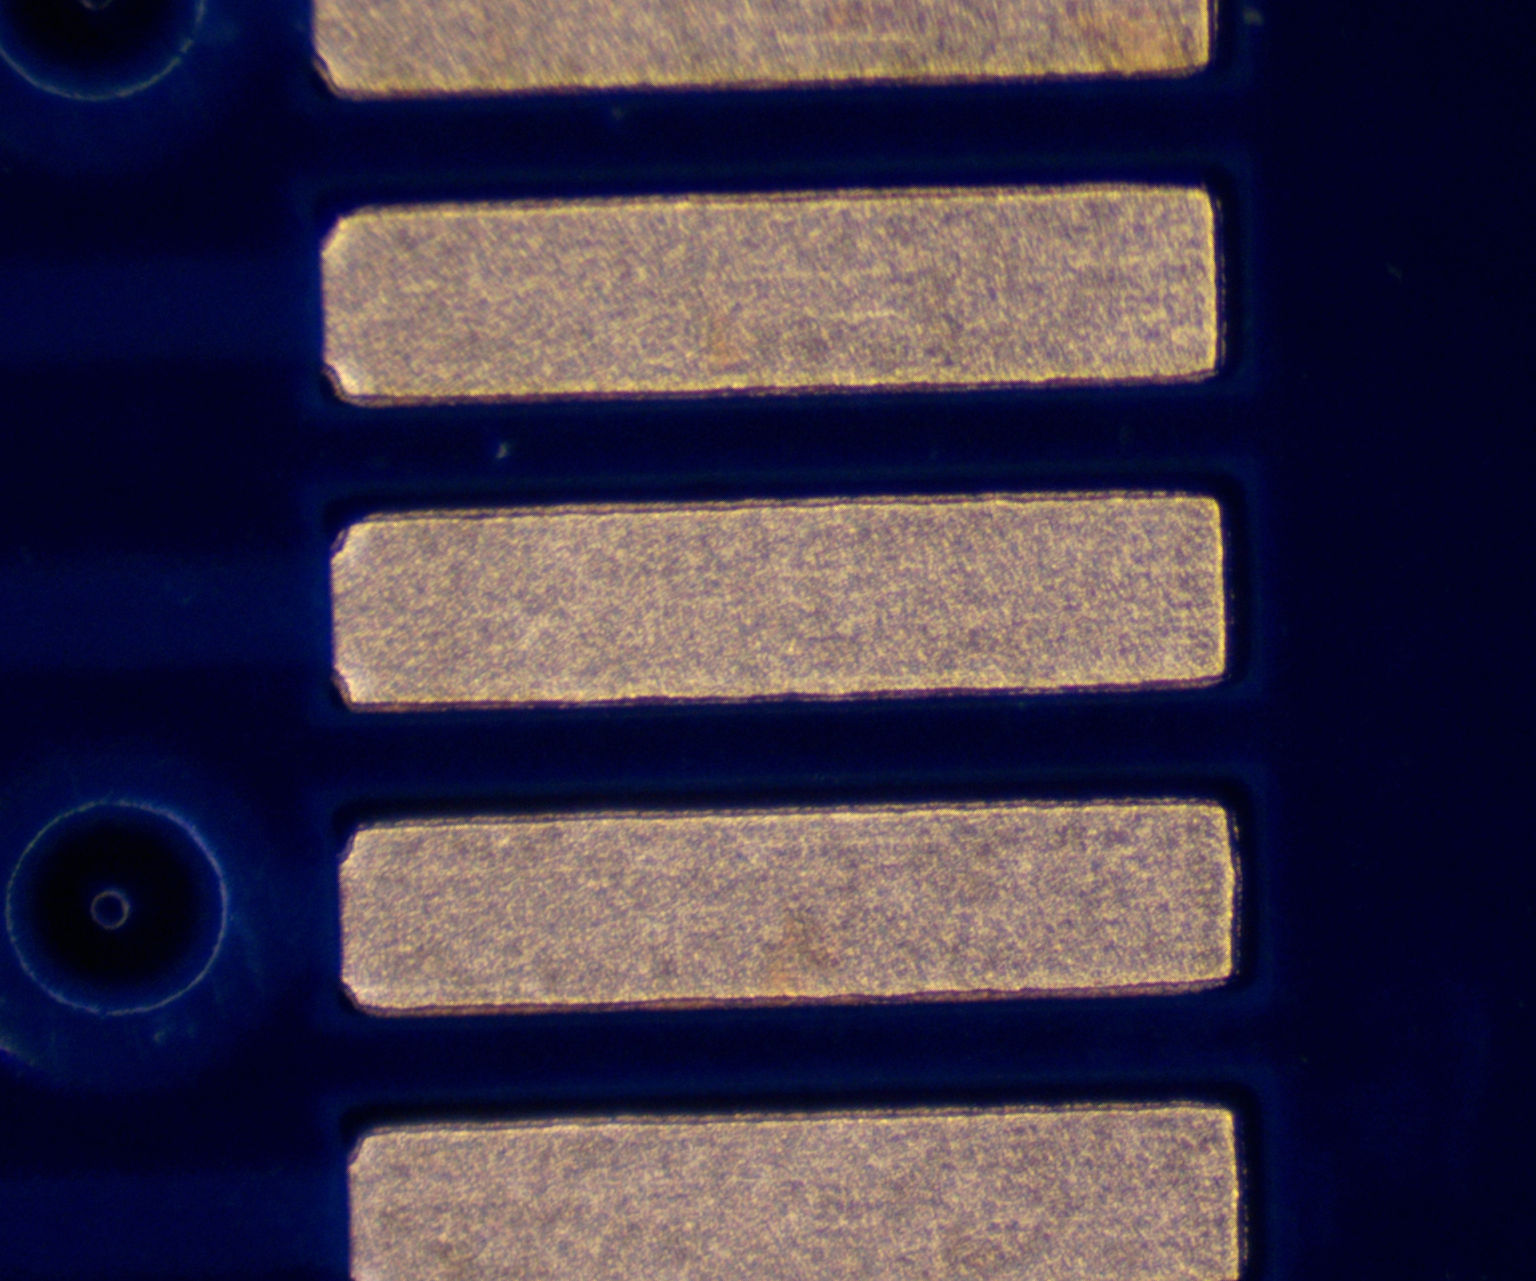
\includegraphics[height=4cm,keepaspectratio]{enig.jpg}
\end{center}
\end{frame}

\begin{frame}
\frametitle{Intermetallic Compounds}
\begin{itemize}
\item Cu, Sn, etc are \emph{soluble} in molten solder!
\item When molten solder is applied to a surface, \emph{diffusion} takes place between the surface and solder
\item The resulting \emph{intermetallic compound} (IMC) bonds strongly to both the solder and component.
\item No IMC = no solder joint (e.g. Sn based solder on Al surface)
\item IMC is, unfortunately, more brittle than bulk solder
\end{itemize}
\end{frame}

\begin{frame}
\frametitle{Oxidation}
\begin{itemize}
\item Metals like to form oxides, esp. when heated
\item Workpieces and solder wire have ``native oxide" layer
\item Working under inert gas inhibits additional oxidation, but won't remove native oxide
\item Oxides prevent IMC formation and free flow of molten solder
\end{itemize}
\begin{center}
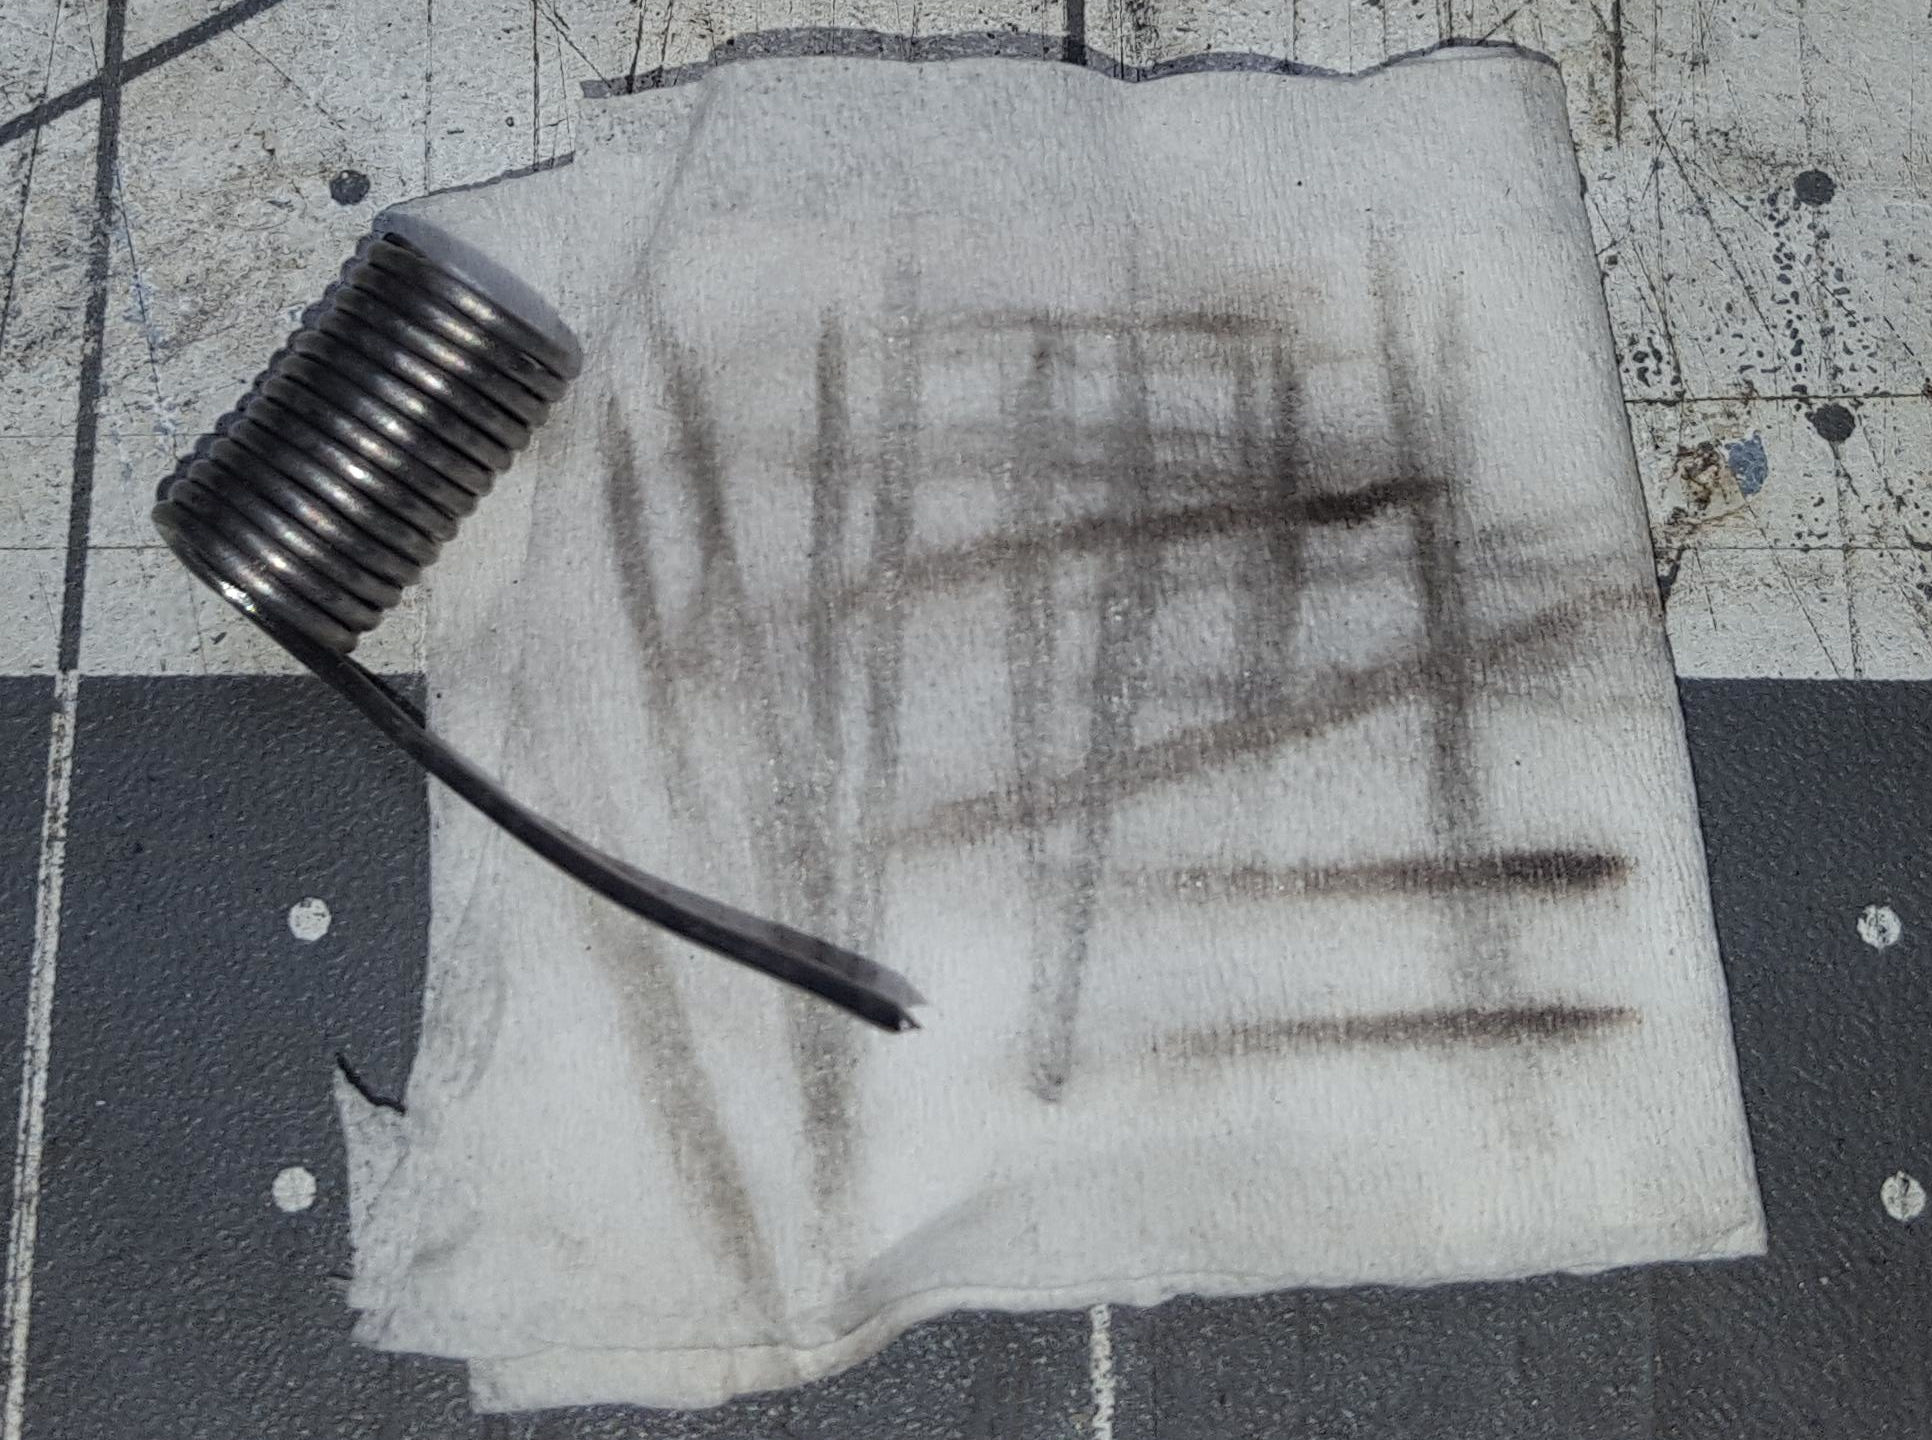
\includegraphics[width=4cm,keepaspectratio]{solder-oxidation.jpg}
\end{center}
\end{frame}

\begin{frame}
\frametitle{Soldering Fluxes - Function}
\begin{itemize}
\item Remove native oxide from surfaces
\item Prevent oxidation of molten solder
\item Strong reducing agents - oxidize rapidly when heated in air
\end{itemize}
\end{frame}

\begin{frame}
\frametitle{Soldering Fluxes - Types}
\begin{itemize}
\item Natural rosin or synthetic compounds
\item Paste, gel, foam, and liquid forms available
\item More active fluxes tend to leave more corrosive residue
\item Less active fluxes may not need cleaning at all
\end{itemize}
\begin{alertblock}{Safety note}
Long-term exposure to flux vapors can trigger allergic reactions or cause asthma. Avoid inhaling flux smoke.
\end{alertblock}
\end{frame}

\begin{frame}
\frametitle{Flux Core Solder Wire}
\begin{itemize}
\item Most solder has 0.5-3\% flux (by weight) in the core
\item Eliminates need to manually add flux to every joint
\item Additional flux may still be needed in some cases
\end{itemize}
\begin{center}
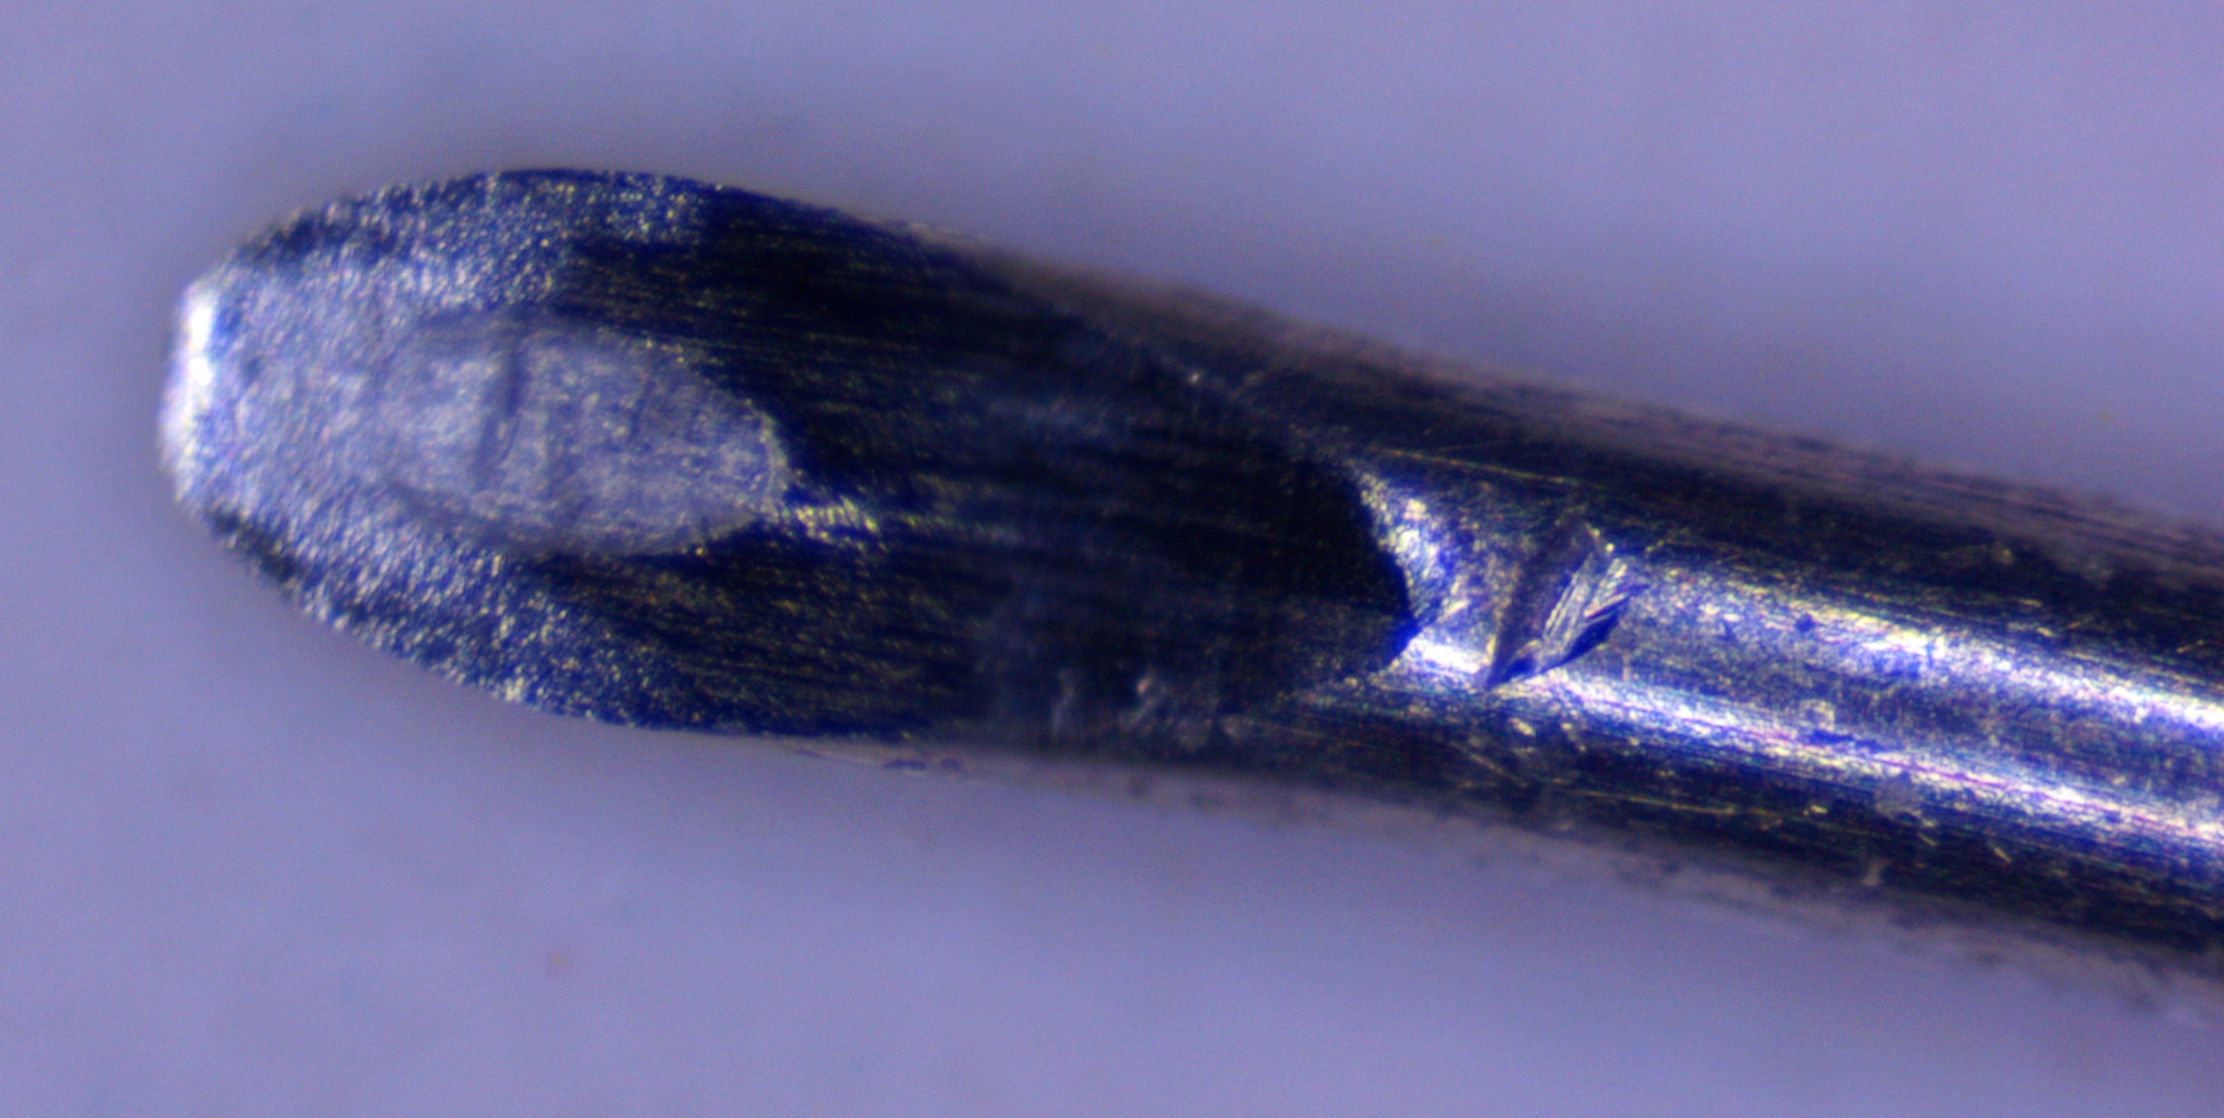
\includegraphics[width=6cm,keepaspectratio]{flux-core.jpg}
\end{center}
\end{frame}

\begin{frame}
\frametitle{Solder Paste}
\begin{itemize}
\item Tiny spheres of solder suspended in sticky flux
\item IPC J-STD-005 type specifies sphere diameter
\item Type 3 (25-45 $\mu m$) and 4 (20-38 $\mu m$) most common
\item Usually stenciled, can also apply with syringe
\end{itemize}
\begin{center}
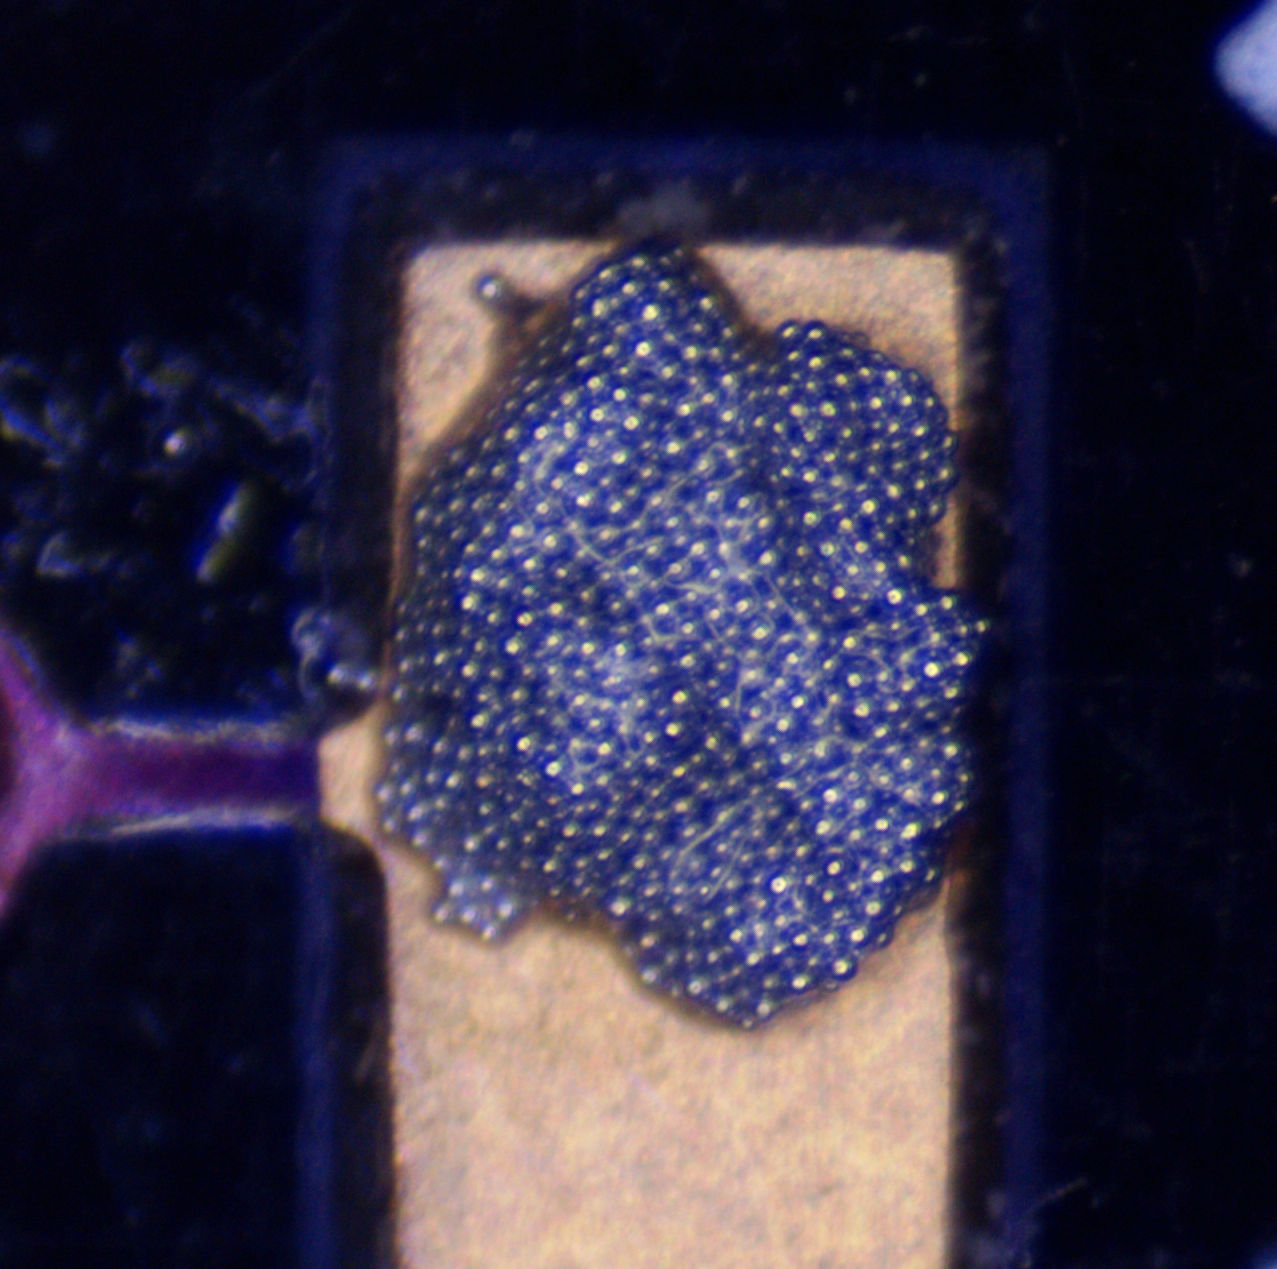
\includegraphics[height=3cm,keepaspectratio]{solder-paste.jpg}
\end{center}
\end{frame}

\begin{frame}
\frametitle{Soldering Processes}
We can classify soldering processes by the heat source used.
\begin{itemize}
\item \textbf{Iron soldering} \\
A heated metal tip provides heat to the joint by \emph{conduction}
\item \textbf{Reflow soldering} \\
Non-contact heating using \emph{convection} or \emph{radiation} in an oven or with a hand-held tool
\end{itemize}
\end{frame}

\begin{frame}
\frametitle{Anatomy of a Soldering Iron}
\begin{itemize}
\item Insulated handle
\item Heat source
\item Tip
\end{itemize}
\begin{center}
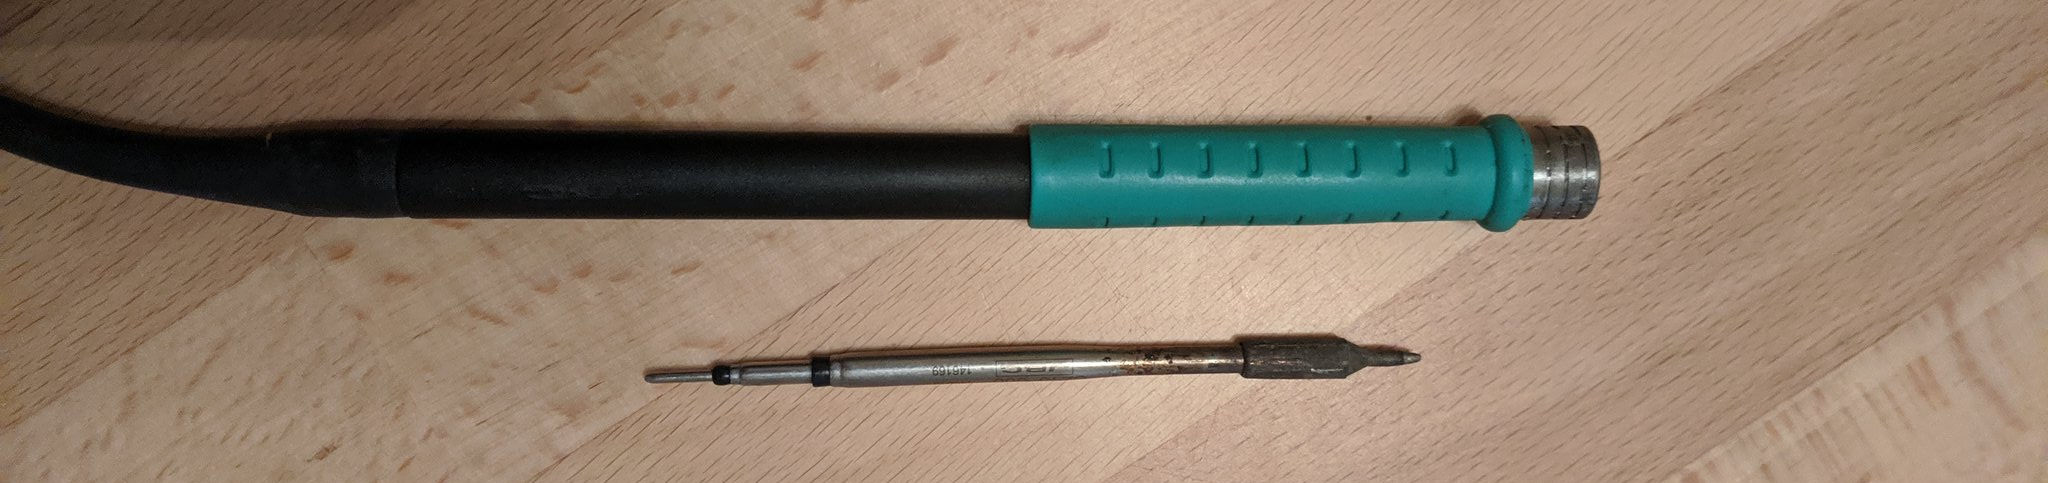
\includegraphics[width=10cm,keepaspectratio]{anatomy.jpg}
\end{center}
\end{frame}

\begin{frame}
\frametitle{Butane Heating}
\begin{itemize}
\item Portable, but poor temperature control
\item Useless for precision work
\end{itemize}
\begin{center}
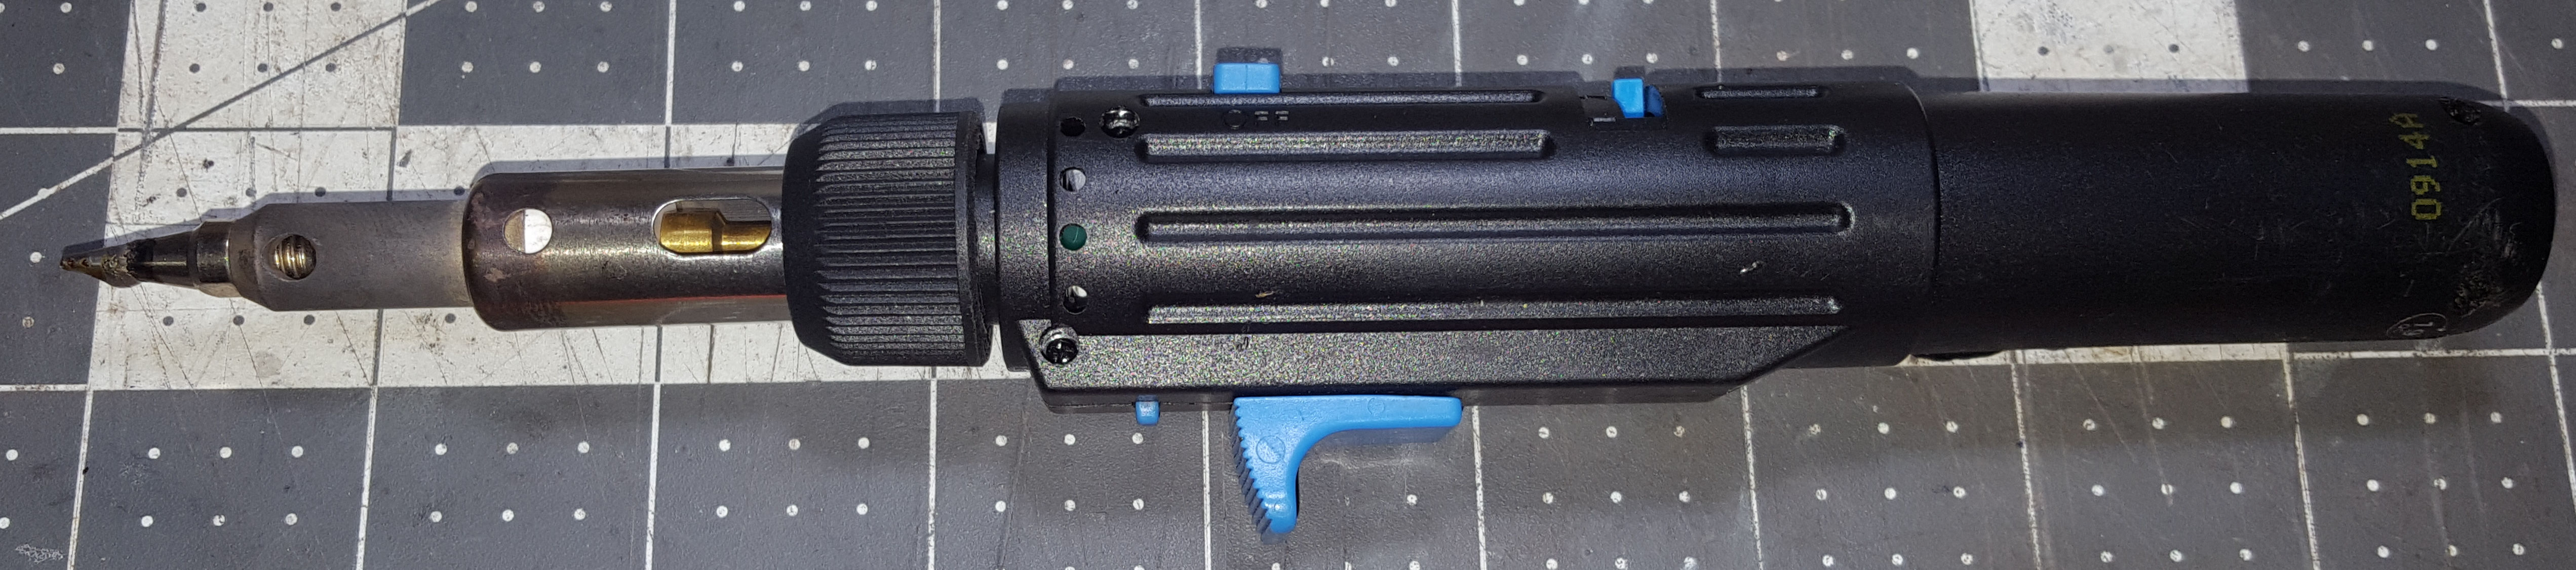
\includegraphics[width=8cm,keepaspectratio]{butane-1.jpg} \\
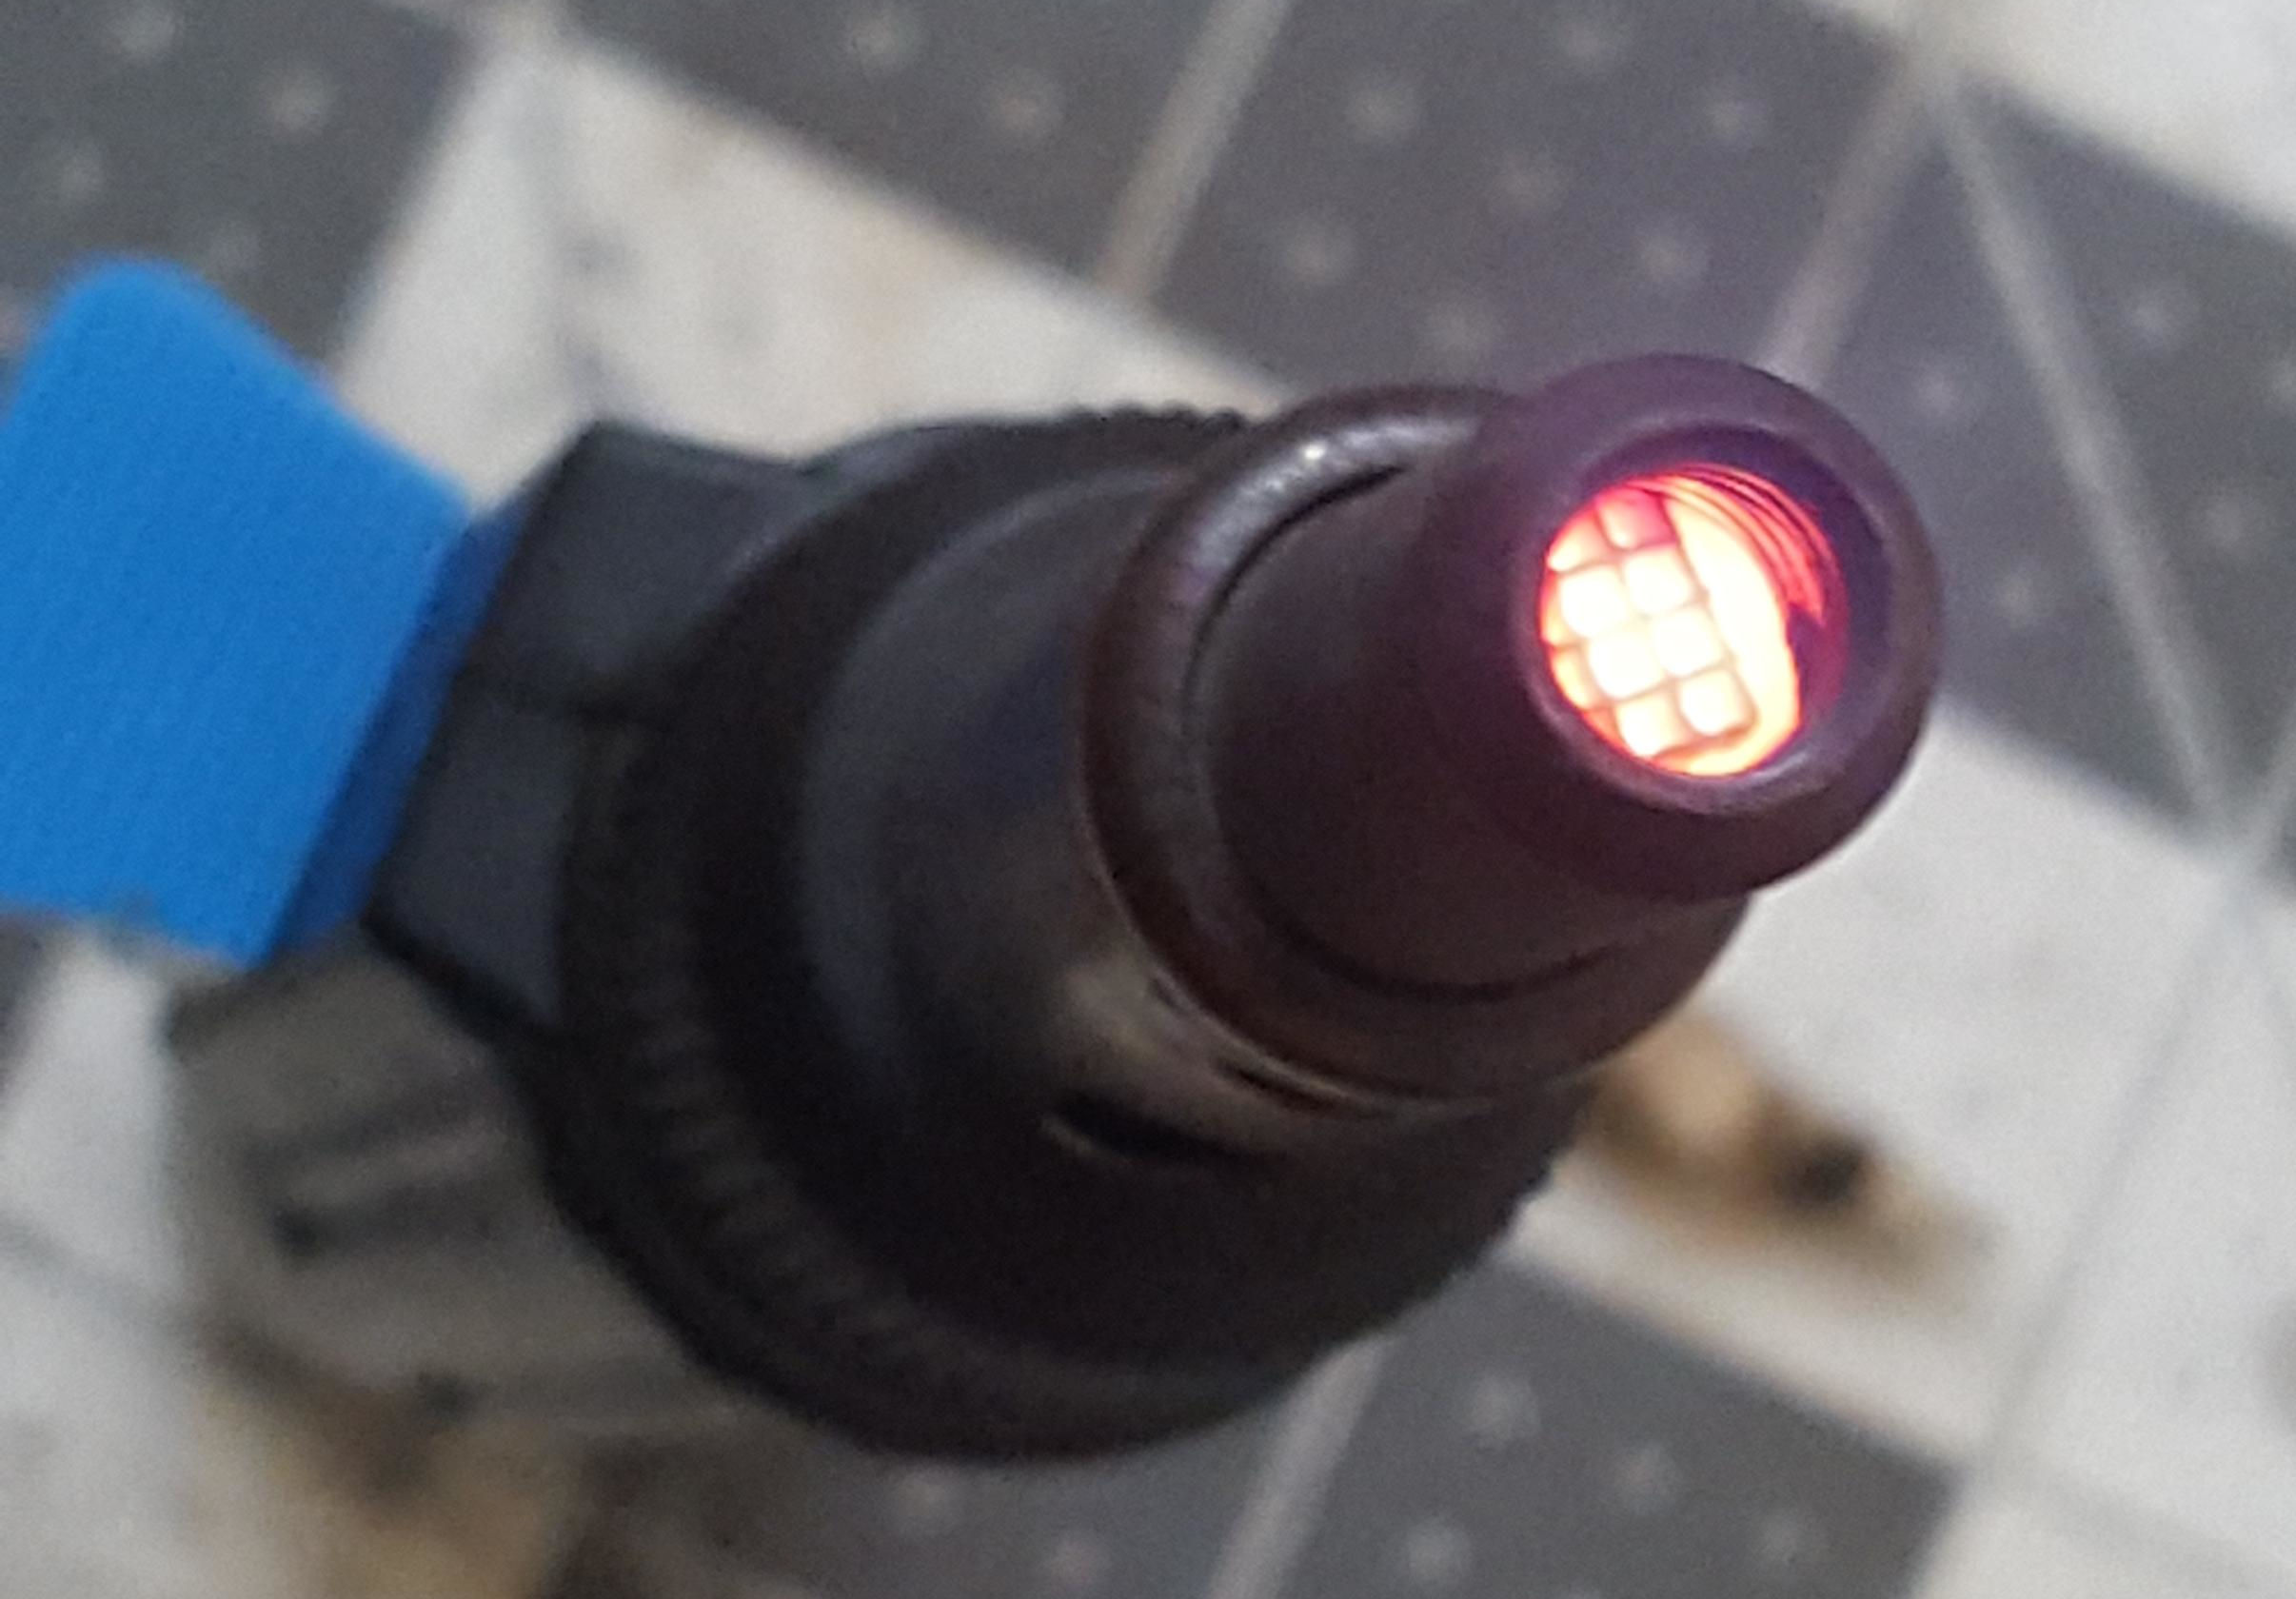
\includegraphics[width=4cm,keepaspectratio]{butane-2.jpg} \\
\end{center}
\end{frame}

\begin{frame}
\frametitle{Uncontrolled 120V Iron}
\begin{itemize}
\item Heating element is fed directly from mains power
\item Usually a coil of nichrome wire
\item No temperature control whatsoever
\item Not useful for modern PCBs
\end{itemize}
\begin{center}
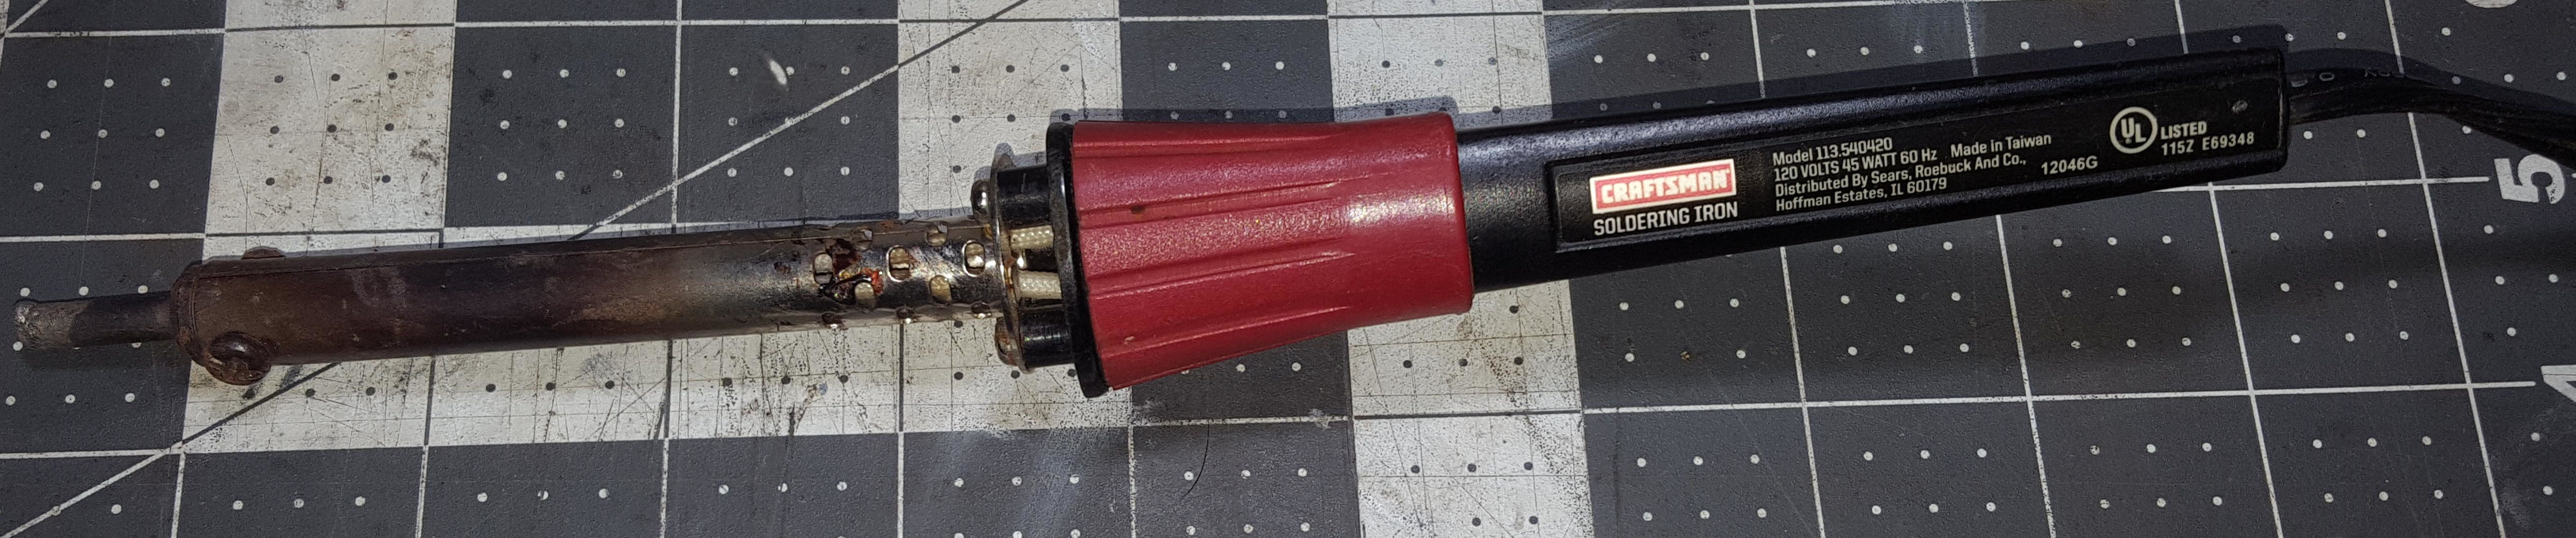
\includegraphics[width=8cm,keepaspectratio]{uncontrolled-iron.jpg} \\
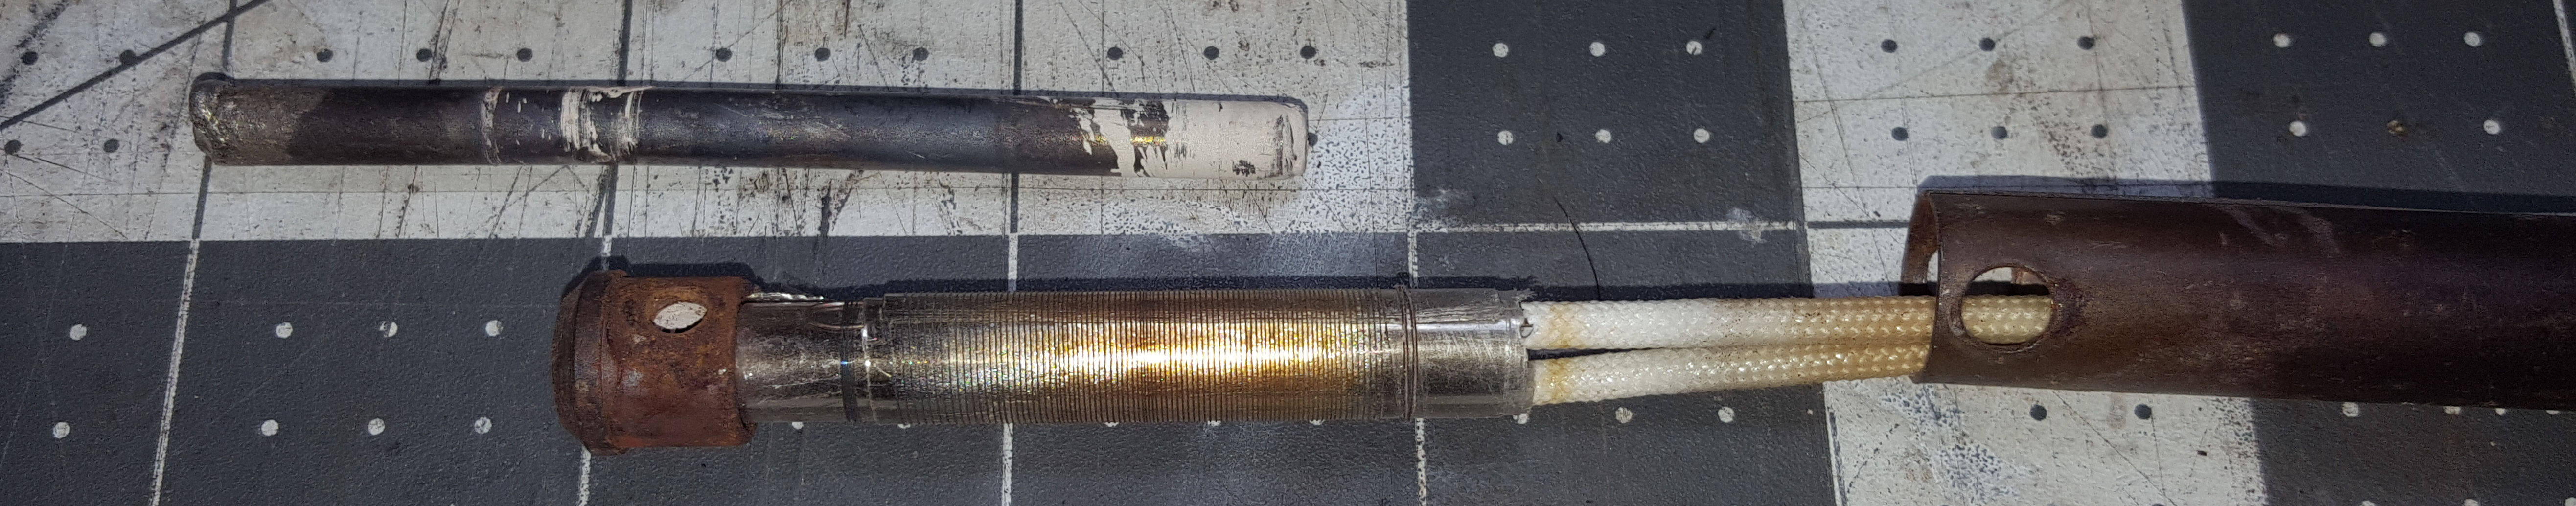
\includegraphics[width=8cm,keepaspectratio]{nichrome-heater.jpg}
\end{center}
\end{frame}

\begin{frame}
\frametitle{Digitally Controlled DC Iron}
\begin{itemize}
\item Typically a ceramic heating element
\item Thermocouple embedded in heater goes to base station
\item Base varies voltage/current to maintain target temperature
\end{itemize}
\begin{center}
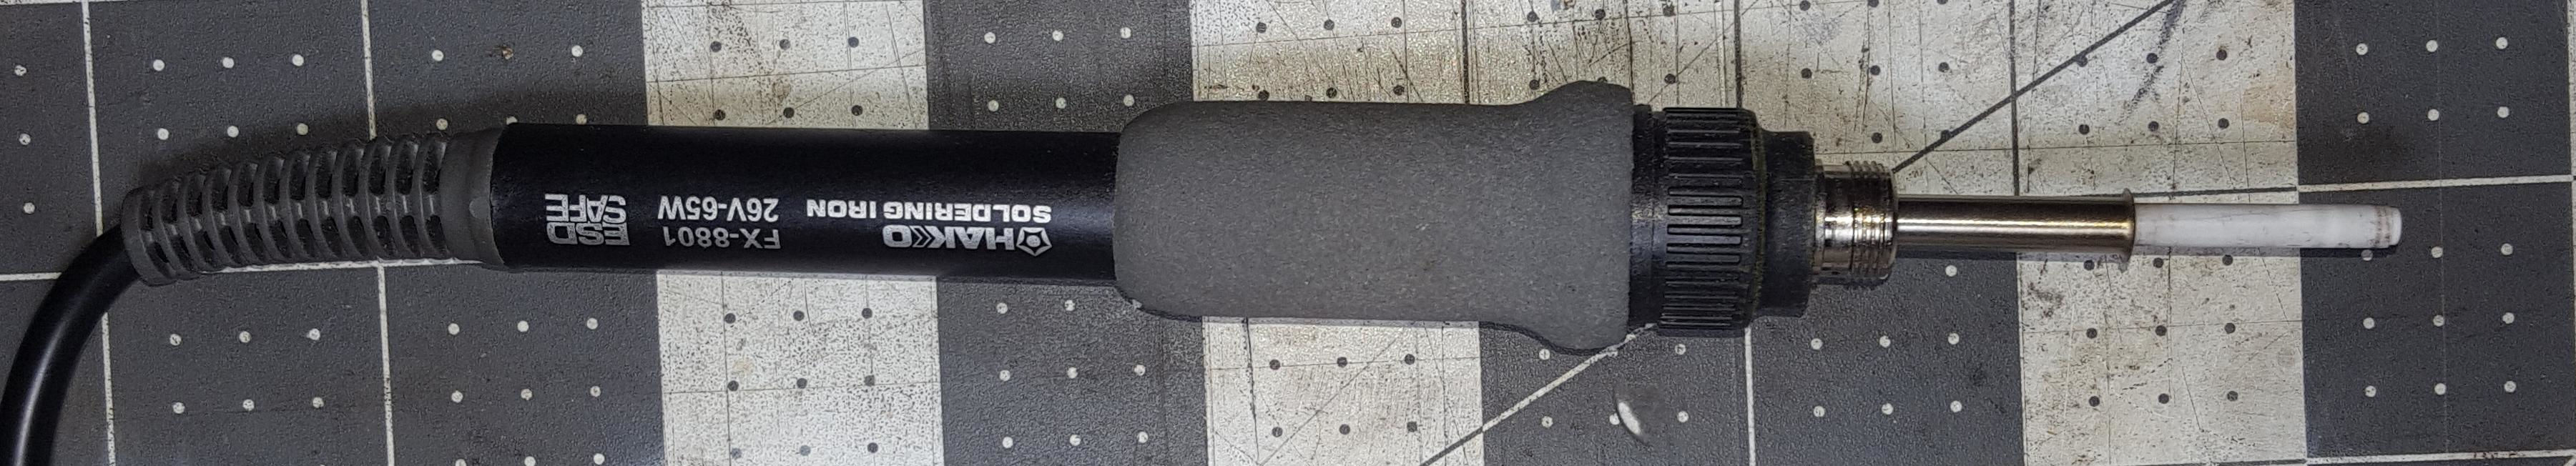
\includegraphics[width=8cm,keepaspectratio]{ceramic-heater.jpg} \\
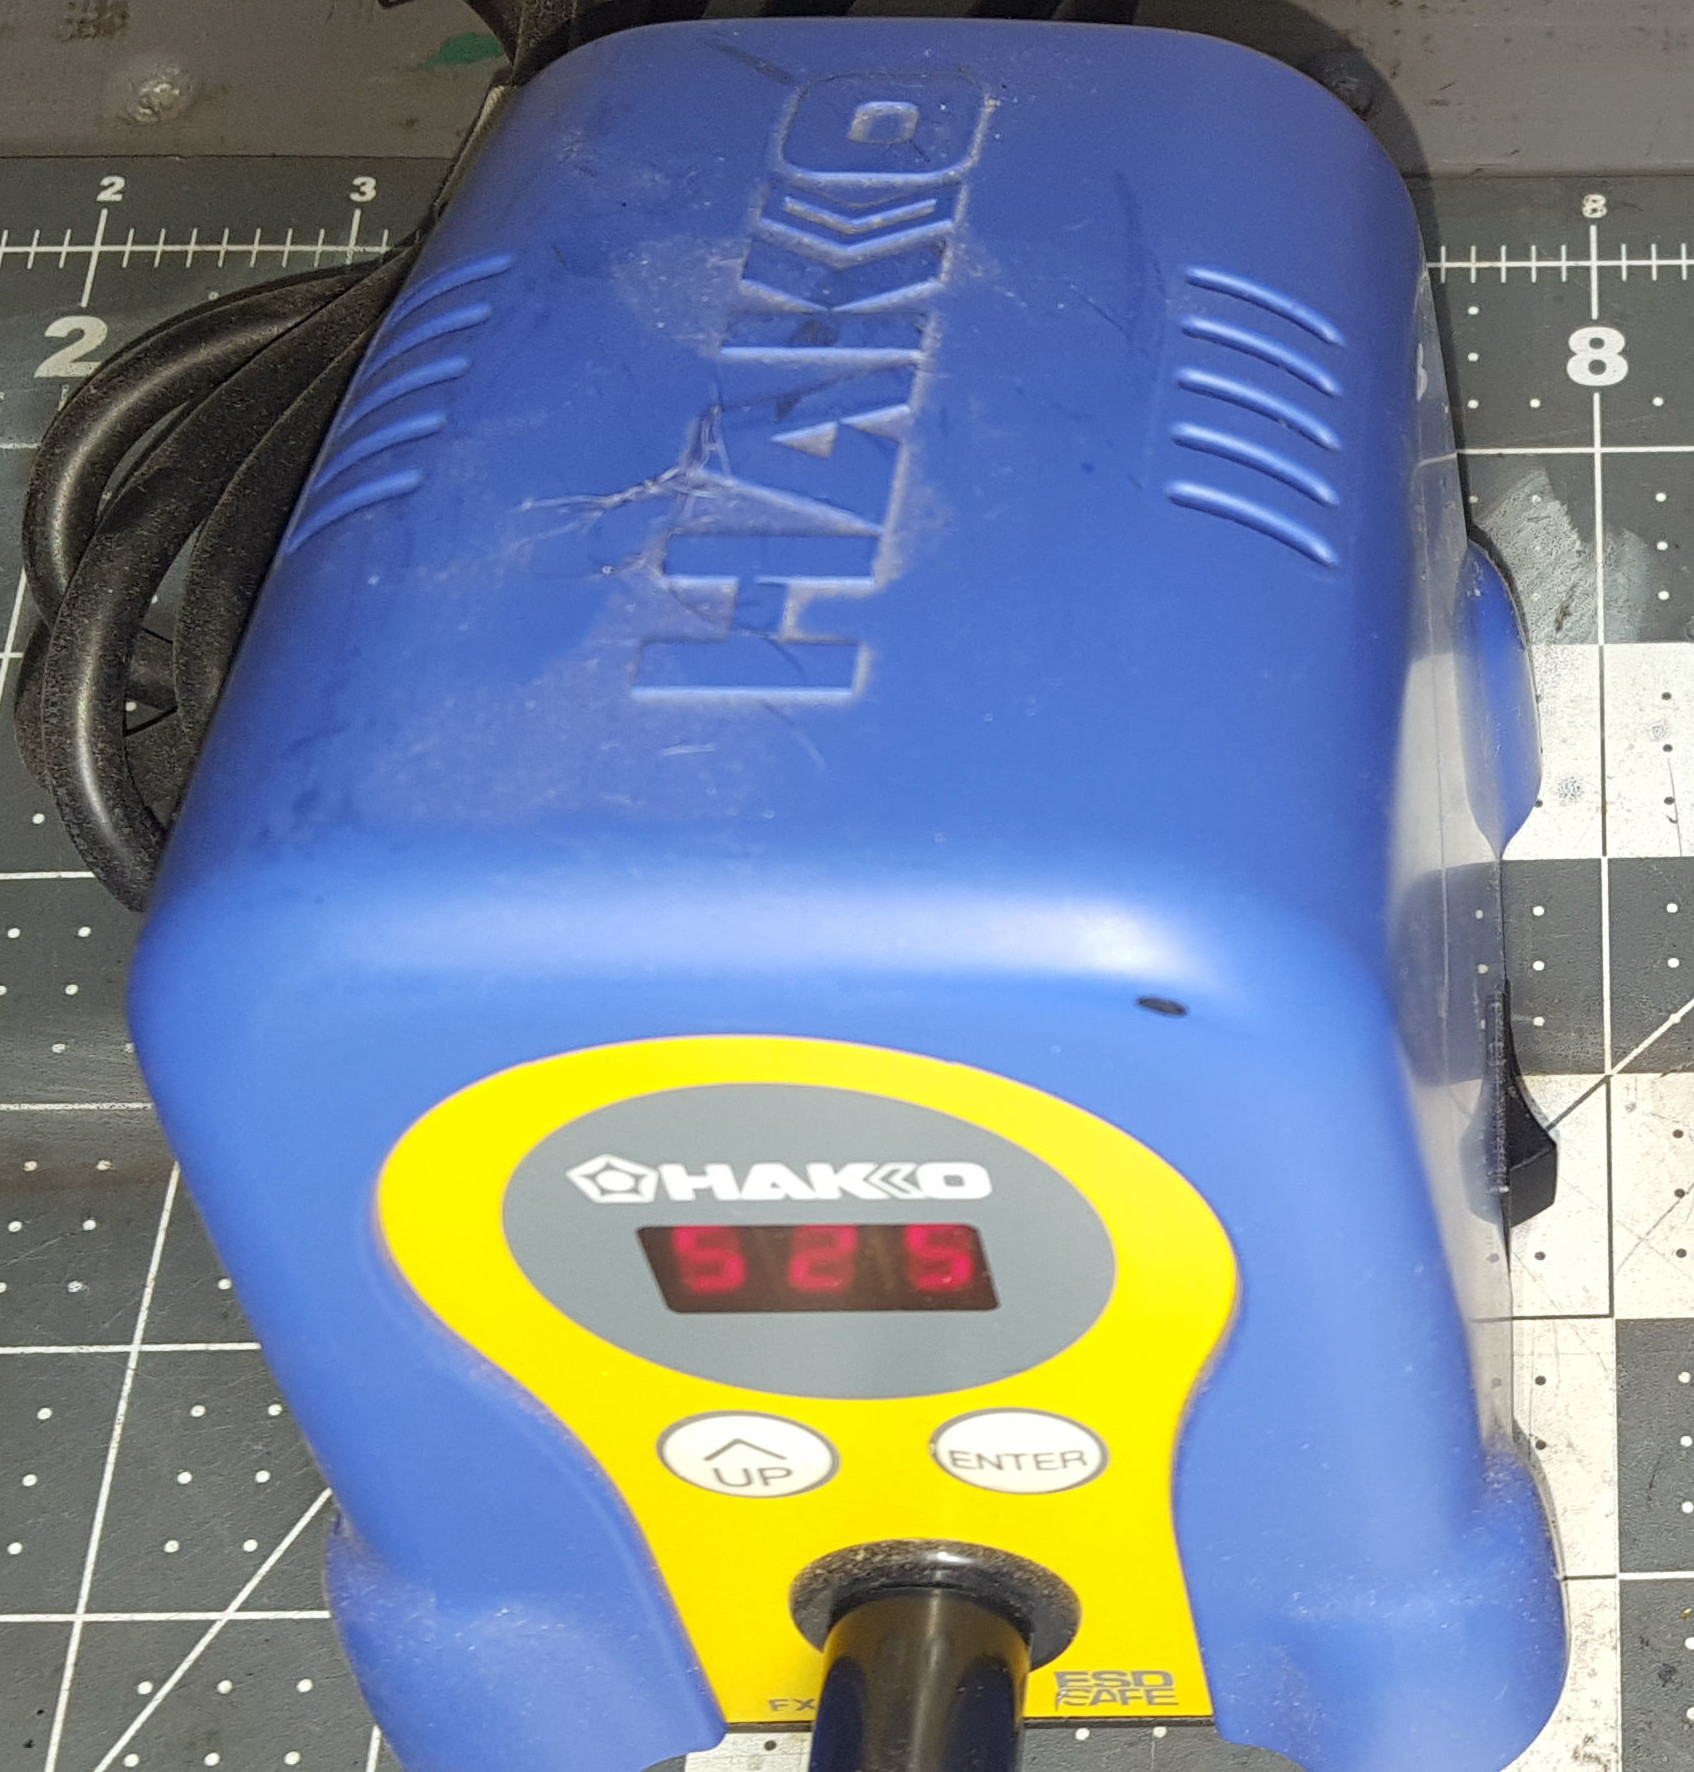
\includegraphics[height=3cm,keepaspectratio]{base-station.jpg}
\end{center}
\end{frame}

\begin{frame}
\frametitle{Curie Point Iron}
\begin{itemize}
\item Base station supplies RF power to a coil
\item Tip inductively couples to coil and self-heats
\item Tip loses magnetism at Curie point and starts cooling
\item Temperature inherently self-regulates
\item Extremely stable, but non-adjustable, temperature
\end{itemize}
\begin{center}
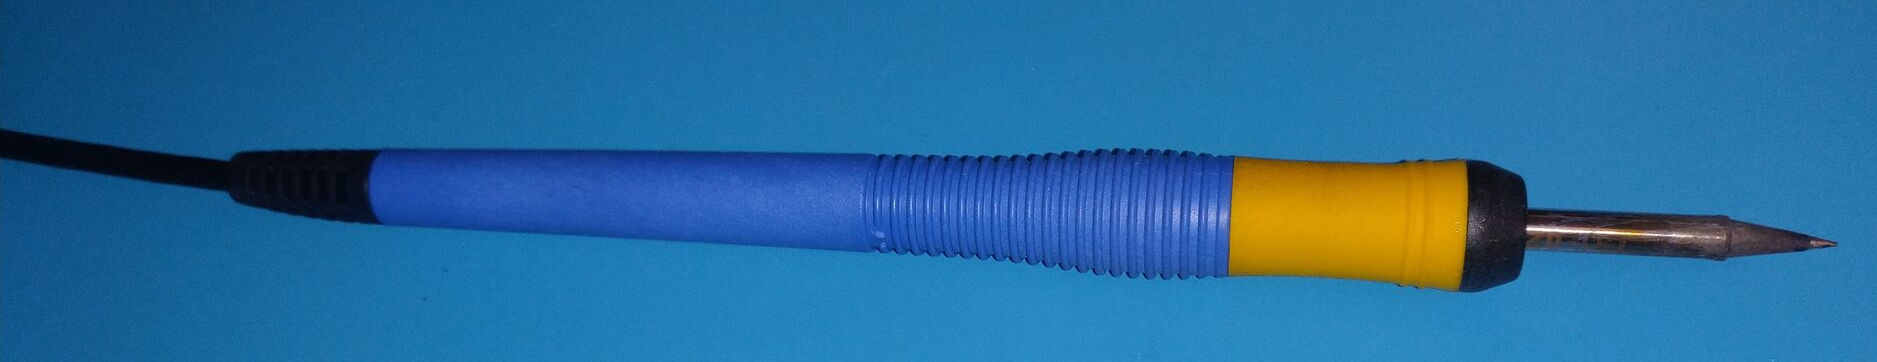
\includegraphics[width=8cm,keepaspectratio]{curie-iron.jpg}
\end{center}
\end{frame}

\begin{frame}
\frametitle{Acknowledgements}
\begin{itemize}
\item Iron anatomy photos - @tawrbo and @Claude1079
\item Oxidized coin - kcrow
\end{itemize}
\end{frame}

\begin{frame}
\frametitle{Questions?}
\end{frame}

\end{document}
